\chapter{Schrodinger equation}
 At the turn of twentieth century ,classical physics which had been quite unstable ,was seriously challenged by two major fronts such as relativistic domain and microscopic domain. In 1905 Einstein's theory of relativity showed that the validity of the Newtonian mechanics ceases at high speeds.As soon as the new experimental technique was developed to the point of probing atomic and sub atomic stuctures it turns out that classical physics fails miserably in providing proper explanantion of several newly discovered phenomena like blackbody radiation,photoelectric effect ,atomic stability and atomic spectroscopy.
  \par The first real break through came in 1900 when Max Plank introduced the concept of the quatum of energy postulating that the energy exchange between radiation and surroundings takes place in descrete or quantized amounts .Which gives accurate explanation to blackbody,photoelectric effect etc.In 1905 Einstein provided poerful consolidation to Plank's quantum concept. In trying to understand photoelectric effect ,Einstein recognized that Plank's idea of quandization of the electromagnetic waves must be valid for light as well.The series of breakthrough due to Plank, Einstein,Bohr and compton gave both theoretical foubdation as well as the conclusive experimental confirmation for the particle aspects of the waves.That is ,the cocepts that waves exhibits particle behaviour at the microscopic level.
  \par In 1923 another new powerful concept that classical physics could not reconcile:He postulated that not only does radiation exhibits particle like behaviour but conversly ,material particle themselves display wave like behaviour.
  \par Quantum mechanichs is the theory that describes the dynamics of matter at the microscopic level.There are two independent formulation of quantum mechanics.The first called matrix mechanics developed by Heisenberg to desribe atomic structure starting from observed spectral lines.The second formulation called wave mechanics was due to Schrodinger ;it is a generalization of the debroglie postulates.
  \section{Wave particle duality}
    According to classical physics ,a particle is characterized by an energy E and a momentum P,whereas a wave characterized by an amplitude and and a wavevector $\vec{k}(\vec{k}=2\pi/\lambda)$ that specifies the direction of the propagation of the wave.Particle and waves exhibits entirely different behaviours;for instance the particle and wave properties are mutually exslusive.We should note that waves can exchange any amount energy with particles.
  \section{PARTICLE ASPECTS OF RADIATION}
  In this section we are going to find how classical physics led to its failure in explaining number of microscopic phenomena such as blackbody radiation ,the photoelectric effect and the compton effect .As it turns out these phenomena could only be explained by by abandoning the concepts of classical physics and introducing a new concept:the particle aspects of radiation.
  \subsection{Blackbody Radiation}
  {\textbf{\large Blackbody:}}\\\\
  A black body, by definition, is an object which absorbs all radiation that falls on it. Since it does not reflect any light, it appears black. In a laboratory, one could approximate a blackbody by a cavity with highly polished walls. If the walls of the cavity has a small hole, any radiation that enters through the hole gets trapped in it. Stars may also be approximated as black bodies as any radiation directed at them gets absorbed.\\\\
  Every  body at constant temperature will emit radiation with a frequency depends up on the temperature of the body. At room temperature most of the radiation is in the infrared part of the spectrum and hence invisible. A hot metal piece will emit visible light an its colour changes from red to yellow to white as it become hotter and hotter. To study the radiation emitted by a hot body , it is convenient to consider an ideal body  which absorbs all the radiation , of any frequency incident on it. Such a body is called blackbody  ,which reflect nothing at all. We introduced the ideal black body to study the thermal radiation is that we can now disregard the precise nature of the radiation, since all black bodies behaves identically.\\
  \begin{figure}[H]
  	\centering
  	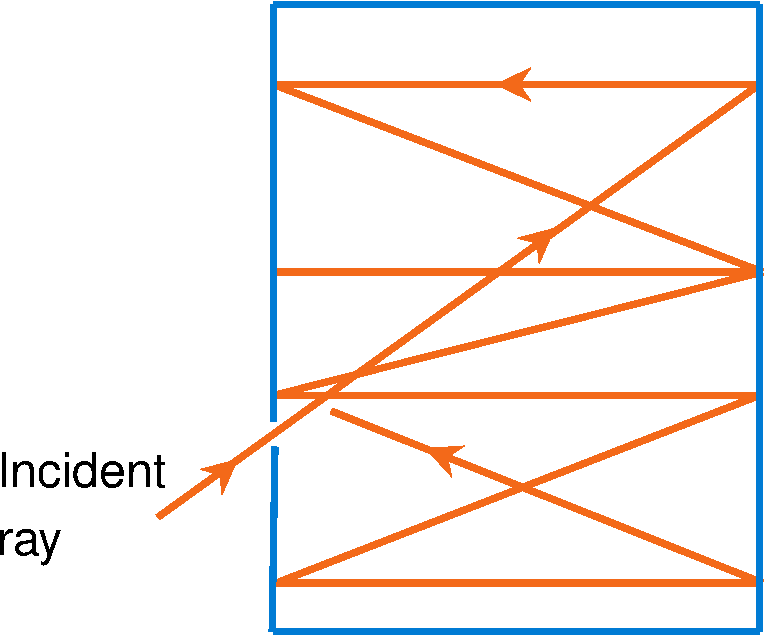
\includegraphics[height=4cm,width=5cm]{30-crop}
  	\caption{Black body radiation}
  	\label{Black body radiation}
  \end{figure}
  If we consider a cavity with ahole  as in figure.\ref{Black body radiation}, Any light entering through the hole is trapped in the cavity undergoes continues reflection and absorbtion until it is finally absorbed. So the cavity wall is constantly emitting and absorbing radiation. These radiation is called blackbody radiation. Experimentally we study the blackbody radiation by examining the radiation coming through the hole in the cavity. The result agree with the observed one.
  \subsubsection{The Ultraviolet Catastrophe}
  The observed spectrum of a black body radiation is given below.
  \begin{figure}[H]
  	\centering
  	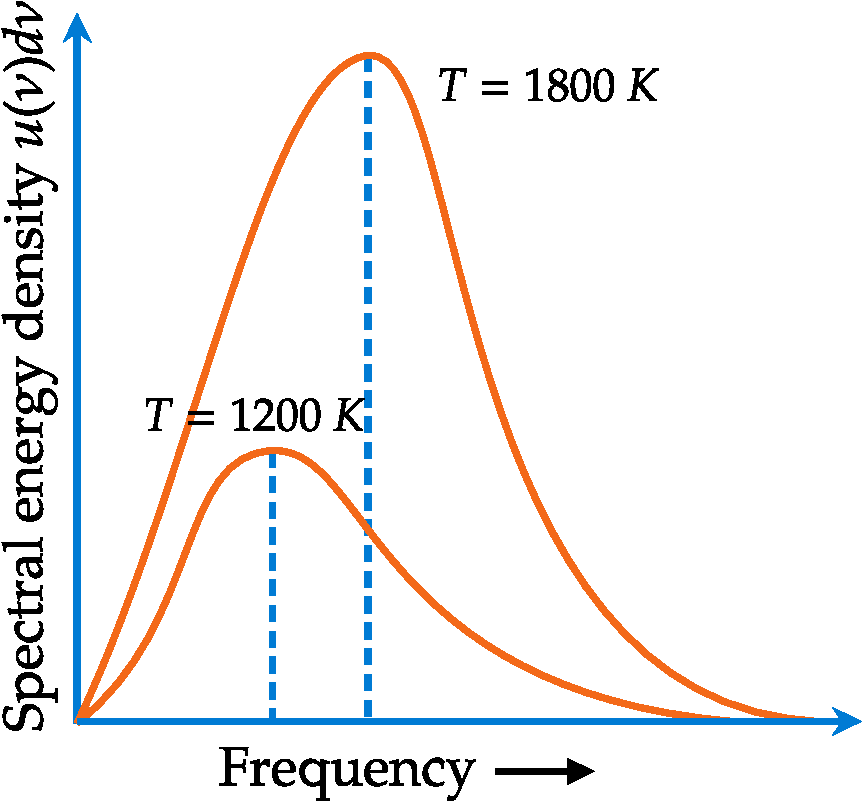
\includegraphics[height=5cm,width=6cm]{01-crop.pdf}
  	\caption{Ultraviolet Catastrophe}
  	\label{Ultraviolet Catastrophe}
  \end{figure}
  First theoretical expression for energy density is given by 
  Rayleigh and Jean. They assumed that the light in the cavity forms standing waves with node occurs at each reflecting surface. The no. of standing waves per unit volume, that is density of standing waves $G(\nu) d \nu$ is given by,
  \begin{center}
  	\framebox{
  		\parbox[t][0.75cm]{4cm}{
  			
  			\addvspace{0.2cm} \centering 
  			
  			$G(\nu) d \nu=\frac{8 \pi \nu^{2} d \nu}{c^{3}}$} }
  \end{center}
  Where $\nu$ is the frequency, $c$  the speed of light. Thus density of standing wave is directly proportional to the square of frequency according to them. The expression for energy density is given by multiplying $G({\nu}) d \nu$ with average energy per standing wave \  $(\bar{\varepsilon})$, so,$$u(\nu) d \nu=G(\nu) d \nu \times \bar{\varepsilon} .$$
  We already know that the EM waves are produced by oscillating electric charge in the cavity. For a body at constant temperature the average energy per degree of freedom is given by, $$\frac{1}{2}KT \ -\text{ Equipartitian theorem.}$$ 
  A one-dimensional harmonic oscillator has two degrees of freedom, one that corresponds to its kinetic energy and one that corresponds to its potential energy. Because each standing wave in a cavity originates in an oscillating electric charge in the cavity wall, two degrees of freedom are associated with the wave and it should have an average energy of $2\left(\frac{1}{2}\right) k T$.
  \begin{align*}
  \text{So average energy} \quad\bar{\epsilon}&=2 \times \frac{1}{2} {KT}={KT}\\
  \therefore \text{Energy density,}\\
  u(\nu) d \nu&=G(\nu) d \nu \times K T\\
  u(\nu) d \nu&=\frac{8 \pi K T \nu^{2}}{c^{3}} d x \Rightarrow\text{ Reyleigh-Jean formula}\\
  \text{That is, }\quad u(\nu) d\nu &\text{ is proportional to } \nu^{2}\\
  \end{align*}
  If we plot we will get,
  \begin{figure}[H]
  	\centering
  	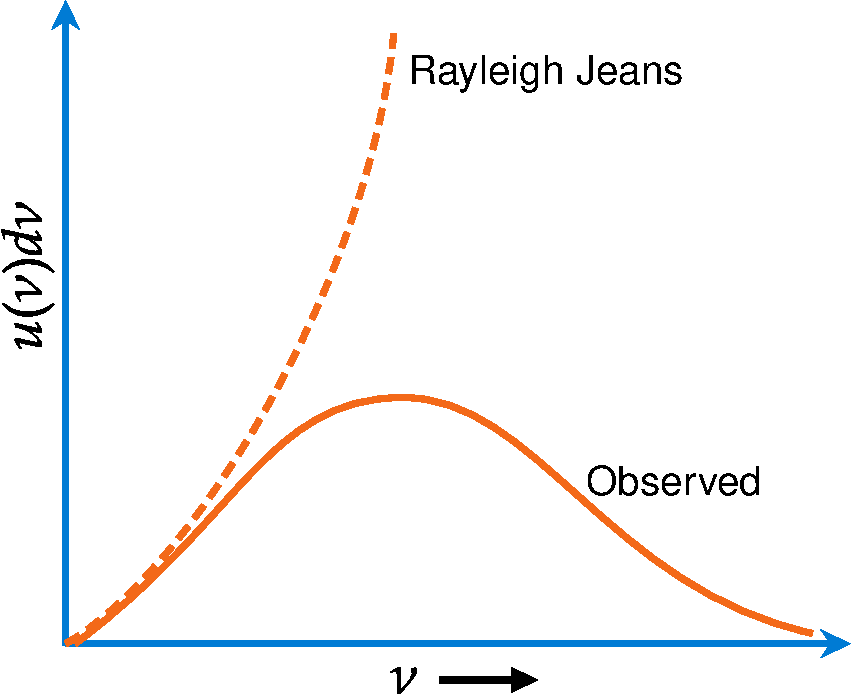
\includegraphics[height=4cm,width=5cm]{1-crop}
  	\caption{}
  	\label{}
  \end{figure}
  \textbf{This discrepency of Rayleigh Jeans formula with the observed spectrum is called ultraviolet catastrophe}. When the frequency increases towards ultraviolet end of the spectrum energy density should increase as $\nu^{2}$ according to Rayleigh - Jeans formula. But actually energy density is decreasing towards $0$, When frequency increases to $\infty$.
  \subsubsection{Plank Radiation Formula}
  The problem of ultraviolet catastrophe is solved by Maxplank by considering that the average energy per standing wave or the energy of a harmonic oscillator is not a continuous value as $KT$ but a descrete value.
  \begin{align*}
  \epsilon_{n}&=n h \nu \qquad n=1,2,3......\\
  \intertext{So average energy per standing wave,}\quad\bar{\varepsilon}&=h \nu \times \frac{1}{e^\frac{h\nu}{KT}-1}\\
  \intertext{ Where $\frac{1}{e^{\frac{h \nu}{KT}}-1}$  is the Bose- Einstein distribution function, which gives the average number of particle in each state of energy $\epsilon$. Therefore energy density of radiation,}
  u(\nu) d \nu&=\frac{8 \pi \nu^{2}}{c^{3}} d \nu \times \frac{h \nu}{e^{\frac{h\nu}{KT}}-1}\\
  &=\frac{8 \pi h}{c^{3}} \frac{\nu^{3} d \nu}{e^{\frac{h\nu}{KT}}-1} \qquad \hspace{0.5cm}\Rightarrow\text{Plank radiation formula}
  \end{align*}
  This result agree with the observed spectrum ie,
  \begin{itemize}
  	\item At high frequencies \quad $h\nu>>KT,\quad\frac{h\nu}{KT} \rightarrow\infty$\\\\ Then,\quad $u(\nu) d \nu \rightarrow 0$ \quad  as observed. 
  	\item At low frequencies
  	\begin{align*}
  	h\nu&<<KT,\frac{h\nu}{KT}<<1\\
  	\text{Then,}\quad e^\frac{h\nu}{KT}&=1+\frac{h\nu}{KT}\hspace{3cm}\because\left[ e^x=1+x+\frac{x^2}{0!}+\frac{x^3}{3!}+.. \right]\\
  	\frac{1}{e^\frac{h\nu}{KT}-1}&=\frac{1}{1+\frac{h\nu}{KT}-1}\\&=\frac{KT}{h\nu}\\
  	u(\nu) d \nu&=\frac{8 \pi h}{c^{3}} \nu^{3}\left(\frac{KT}{h\nu}\right) d \nu\\&=\frac{8 \pi KT }{c^3} \nu^{2} d \nu\\
  	u_{\nu}(\nu)&=\frac{8 \pi h \nu^{3}}{c^{3}} \cdot \frac{1}{\exp \left(\frac{h \nu}{k T}\right)-1}
  	\end{align*}
  	
  \end{itemize}
  At low frequencies plank radiation formula reduces to Reyleigh-Jeans formula. No descrepency at low  frequencies.
  \begin{note}
  	\begin{enumerate}
  		\item $u(\nu)$ is called spectral energy density and has a dimension:\quad $M L^{-1} T^{-1}$
  		\item The spectral frequency in terms of angular frequency $\omega$.\\
  		$$u(\omega)=\frac{\hbar \omega^{3}}{\pi^{2} c^{3}} \cdot \frac{1}{e^{\left(\frac{\hbar \omega}{k T}\right)-1}} $$
  		\item The spectral frequency in terms of wave length $\lambda$
  		$$ u(\lambda)=\frac{8 \pi h c}{\lambda^{5}} \cdot \frac{1}{e^ {\left(\frac{h c}{\lambda k T}\right)-1}}$$
  	\end{enumerate}
  \end{note}
  \subsubsection{Photon}
  \textbf{Planck's  explanation  of  black  body  radiation  was  revolutionary  as  it  suggested  that  atoms  could  exchange energy  only  in  multiples  of  quantum  of  energy. } 
  In this concept light  consist of particles known as \textbf{photon} with energy equal to $h \nu$. So it's total energy is quantized $(h\nu)$ in terms of each quanta photon $(h \nu)$ which is descrete. But according to wave theory, light waves leave a source with their energy spread out continuously through the wave pattern. That is the difference from quantum theory.
  \begin{itemize}
  	\item\textbf{ Energy of Photon}
  	\begin{align*}
  	E&=h \nu, \qquad  \intertext{  $\nu$ is the frequency and $h$ is called the Plancks constant}
  	h&=6.626 \times 10^{-34} \mathrm{J} \cdot \mathrm{S}\\
  	\text{ Dimension of } h&=M L^{2} T^{-2} \times T\\
  	&=M L^{2} T^{-1} \quad  \left(\text  { $h$ has a dimension of angular momentum. }\right) \\ 
  	\text{Now we can define a new quantity,} \  \hbar&=\frac{h}{2 \pi}\\
  	\omega&=2 \pi f\\
  	\therefore E&=\hbar \omega
  	\end{align*}
  	\item \textbf{Momentum of Photon}\\
  	\begin{align*}
  	\intertext{The momentum associated with photon is expressed in terms of wave number , \ $k=\frac{2 \pi}{\lambda}$}
  	p&=\hbar k \qquad \Rightarrow p=\frac{h}{\lambda}
  	\intertext{In relativity total energy can be expressed in terms of momentum and restmass energy as}
  	E^{2}&=P^{2} c^{2}+\left(m_{0} c^{2}\right)^{2}
  	\intertext{ For a photon, rest mass \ $m_{0}$\ is zero.}
  	\therefore E&=P c\\
  	\intertext{ Then momentum,}
  	p&=\frac{E}{c}=\frac{h \nu}{c}
  	\end{align*}
  	\item\textbf{Mass of a photon}
  	\begin{align*}
  	\intertext{Although  a photon have no restmass if it interact with an electron, it acquires a mass, $m$}
  	p&=\frac{E}{c}\\
  	m c&=\frac{E}{c}\\
  	m&=\frac{E}{c^{2}}=\frac{h \nu}{c^{2}}
  	\end{align*}
  \end{itemize}
  \begin{exercise}
  	Find the wave length and frequency of a $1$ kev photon.
  \end{exercise}
  \begin{answer}
  	\begin{align*}
  	E&=1 \times 10^{3} \mathrm{ev}\\
  	E&=10^{3} \times 1.6 \times 10^{-19} \mathrm{~J}\\
  	E&=\frac{hc}{\lambda}\\
  	\lambda&=\frac{hc}{E}=\frac{6.6 \times 10^{-34} \times 3 \times 10^{8}}{10^{3} \times 1.6 \times 10^{-19}}\\
  	&=12.4 \text{\AA}\\
  	\nu &=\frac{c}{\lambda}=\frac{3 \times 10^{8}}{12.4 \times 10^{-10}}\\
  	&=2.42 \times 10^{17} \mathrm{~Hz}
  	\end{align*}
  	
  \end{answer}
  
  \subsubsection{Wien's Displacement Law}
  There is an interesting relationship between the peak wavelength and the temperature at which a blackbody radiates.  For a given temperature, the spectrum of emitted radiation has maximum intensity for a wavelength $ \lambda_{max}$.\\
  We will get the maximum wavelength  by differentianting $u (\lambda
  )$ with respect to $\lambda$,
  \begin{align*}
  \frac{d u(\lambda)}{d\lambda}&=0 \ \text{ at }\  \lambda=\lambda_{max}
  \intertext{At maximas and minimas the first derivative of a function must vanish. After differentiation we will obtain $u (\lambda
  	)$  as,}
  \frac{hc}{KT\lambda_{max}}&=4.965\\
  \lambda_{max}T&=\frac{hc}{4.965}=2.898\times10^{-3}m\cdot K\\
  \lambda_{max}T&=2.898\times10^{-3}m\cdot K\qquad\Rightarrow\text{Wien's displacement law}
  \end{align*}
  Which expresses the emperical fact that the peak in the blackbody spectrum shift to progressively shorter wavelength (higher frequencies) as the temperature  increases.\\
  The shift of that peak is a direct consequence of the plank radiation law. Which describes the spectral brightness of black body radiation as a function of wavelength at a given temperature. However it had been discovered by Wilhelm Wien several years before Max Plank developed that more general equation, and describes the entire shift of the spectrum of blackbody  radiation towards shorter wavelength  as temperature increases.  
  \begin{figure}[H]
  	\centering
  	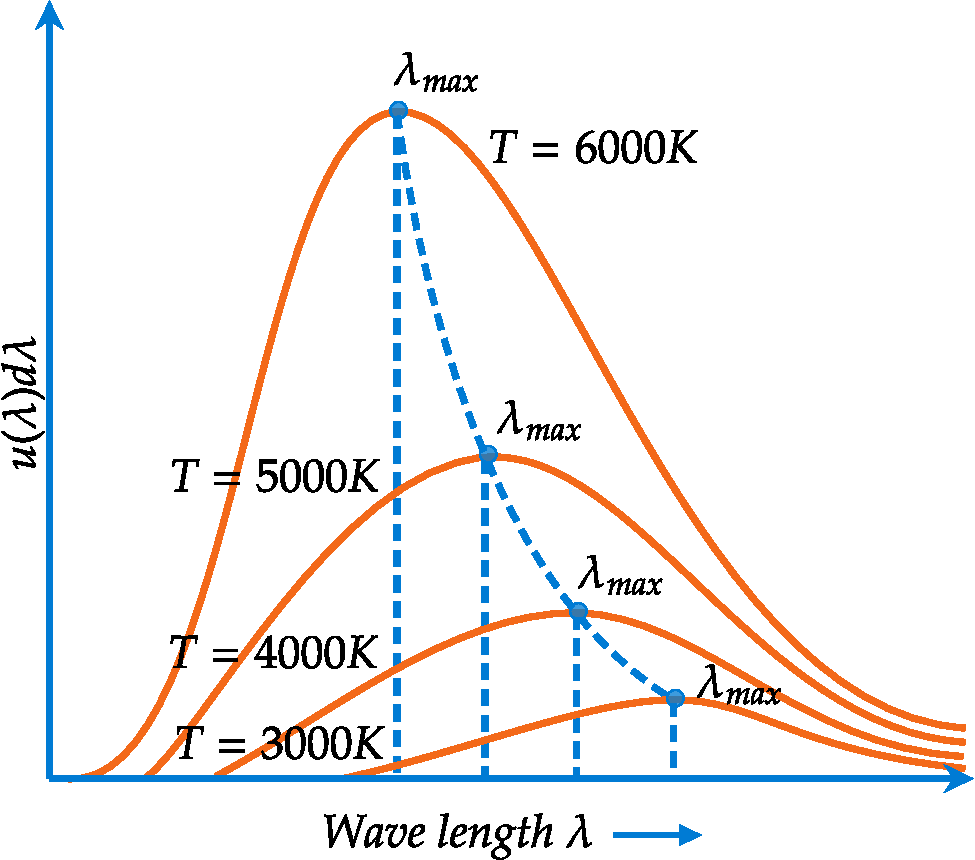
\includegraphics[height=6cm,width=7cm]{5-crop}
  	\caption{}
  	\label{}
  \end{figure}
  \begin{exercise}
  	Find the peak wave length in the spectrum of radiation from a blackbody at a temperature of $500$ \AA. In what part of the em spectrum is this wavelength
  \end{exercise}
  \begin{answer}
  	\begin{align*}
  	\lambda_{max} T&=2.898\times10^{-3}\\T&=500+273=773K\\
  	\lambda_{max}&=\frac{2.898\times10^{-3}}{773}\\
  	3.7\times10^{-3}\times10^{-3}&=3.7\mu m \quad 
  	\left( \text{Mid-infrared region}\right) 
  	\end{align*}
  \end{answer}
  \subsubsection{Stefan-Boltzman Law}
  The total energy density $u$ of the radiation in the cavity is given by,
  \begin{align*}
  u&=\int u(\nu) d x\\&=\frac{8 \pi^{5} k^{4}}{15 c^{3} h^{3}} T^{4}\\&=a T^{4}
  \end{align*}
  $ a $ is a universal constant,\  $a=7.56 \times 10^{-16}$ Since $u$ (Energy density) is proportional to $T^4$, the energy $R$ (Radiation per second per unit area) is also preportional to $T^4$. So ,
  \begin{align*}
  R&\propto T^4,\\
  R&=e\sigma T^4\Rightarrow\text{ Stefan-Boltzmann law }\\
  \intertext{$\sigma$ is called Stefan's constant}
  \sigma&=\frac{ac}{4}=5.670\times10^{.8}W/m^2\cdot K^4
  \intertext{  $ e$ is the emissivity, depends on the nature of the body radiating}
  \end{align*}
  \begin{note}
  	\begin{enumerate}
  		\item
  		\text{a)}\quad$e=0$ \qquad For a perfect reflector.\\\\
  		\text{b)}\quad$e=1$ \qquad (Maximum) For a blackbody (zero reflection).\\\\
  		\text{c)}\quad$e=.07$ \qquad For polished steel.\\\\
  		\text{d)}\quad$e=0.6$ \qquad For oxidized copper and brass.\\\\
  		\text{e)}\quad$e=0.97$\qquad  For black paint.
  		\item $R$ \ is the energy radiated per unit time per unit area. So $R$ can be written as ,
  		$$R=\frac{\text { Power output }}{\text { Surface Area }}$$ 
  	\end{enumerate}
  \end{note}
  
  
  \begin{exercise}
  	A copper sphere $5cm$ in diameter whose emissivity is $0.3$ is heated in a furnace to $400^\circ C$. At what rate it radiate?
  \end{exercise}
  \begin{answer}
  	\begin{align*}
  	R&=\frac{\text{Power}}{\text{Surface area}}\\
  	R&=\sigma e T^4\\
  	\therefore\text{ Power}&=\sigma e T^4\times4\pi r^2\\
  	T&=400+273=673K\\
  	e&=0.3\\
  	\sigma&=5.67\times10^{-8}\\
  	r&=5\times10^{-2}m\\
  	\text{Power rate}&=27.39 W
  	\end{align*}
  \end{answer}
\subsection{Photo Electric Effect}
\textbf{When light certain minimum frequency falls on certain metals, electrons are emitted in all directions from the surface of the metal ,  this phenomenon is called photo-electric effect}. These electrons are called photoelectrons.\\
This was first observed by Hertz during his experiment on em waves. But he did not follow up this observation. The correct explanation of photoelectric effect is given by Einstein using Planck's quantum hypothesis. Einstein put forward a theory of photoelectric effect which suggested that the quantum of energy was not a property associated with the radiation emitted by atoms but is a property of radiation itself.  He assumed that light consist of small packets called photons having energy equal to $h\nu$($\nu$ is the frequency). 
\begin{figure}[H]
	\centering
	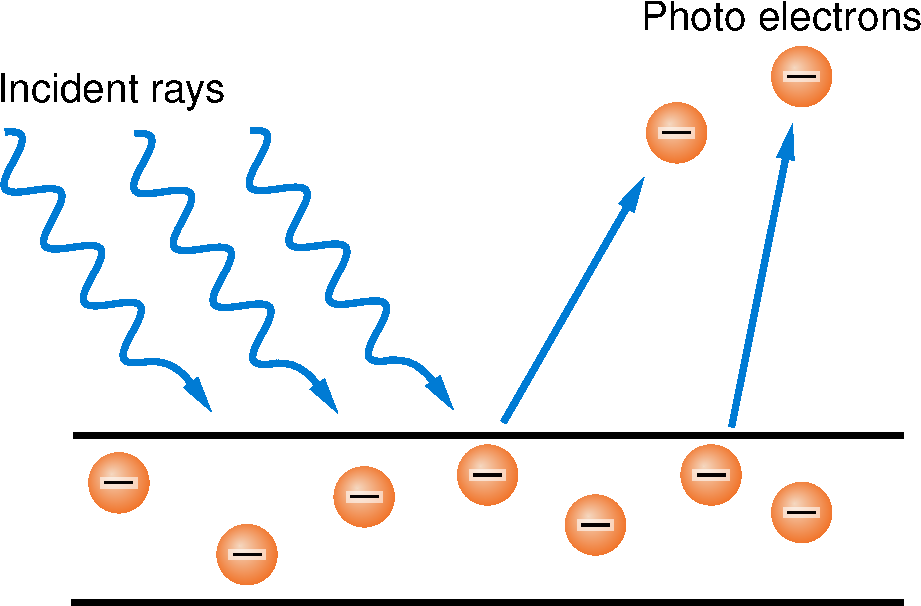
\includegraphics[height=4cm,width=6cm]{Photoelectric}
	\caption{Photo Electric Effect}
	\label{Photo Electric Effect}
\end{figure}
\subsubsection{Experimental setup} 
In the arrangement shown in the figure. \ref{Photoelectric effect} , the wire marked anode is held at positive potential with respect to the curved plate marked cathode.  When light of certain minimum frequency falls on the cathode, electrons are emitted in all directions. These electrons are called photoelectrons. Some of these electrons reach the anode wire which provides a path to the electrons to give rise to a mesurable photo-current . By making the anode more positive with respect to the cathode, more electrons are attracted towards the anode and the photo-current increases. When the anode potential is such that all the emitted electrons reach the anode, any further increase in the anode voltage does not increase current any further.
\begin{figure}[H]
	\centering
	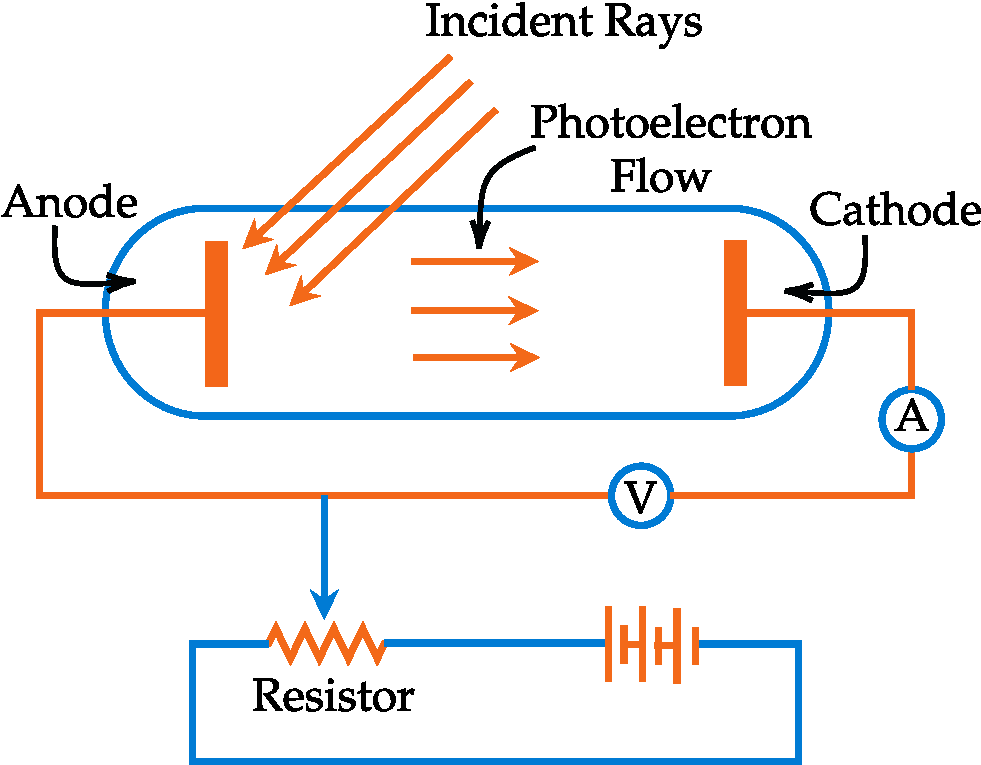
\includegraphics[height=5cm,width=7cm]{17.11-crop}
	\caption{Experimental stup for Photoelectric effect}
	\label{Photoelectric effect}
\end{figure}


Einstein explained the three experimental observation using his hypothesis.\\\\
\textbf{(1)}\quad Because wave energy is concentrated in photon it's not spread out in space (as in classical wave). \textbf{There should be no delay in the emission of photoelectrons}.\\\\
\textbf{(2)}\quad All photons of freqency $\nu$ has the same energy, so changing the intensity of monochromatic light beam will change the no.of photo electrons but not their energies. A bright light yields more photoelectrons than a dim one of the same frequency.
\begin{figure}[H]
	\centering
	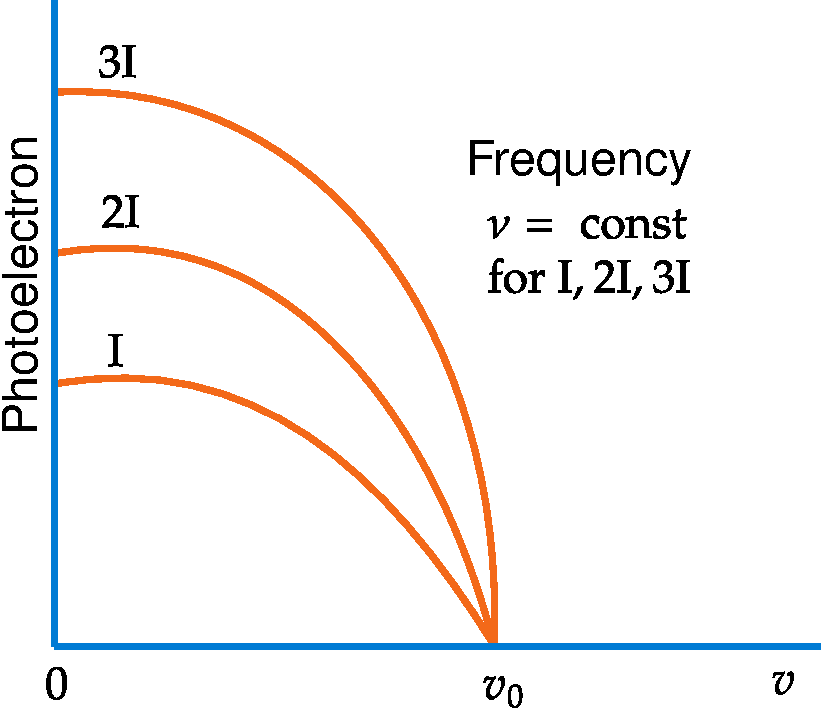
\includegraphics[height=5cm,width=6cm]{6-crop}
	\caption{}
	\label{photo2}
\end{figure}
Where $V_0$ is called \textbf{retarding potential} or \textbf{stopping potential}. Which refers to the voltage difference required to stop electrons from moving between plates during a photoelectric experiment. In order to stop an electron the energy we applied $(eV_0)$ must be equal to the maximum kinetic energy of the photo electron emitted.
$$\therefore ev_0=\frac{1}{2}mV^2=KE_{max}$$
Here in this figure. \ref{photo2},\  all the three light $(I,2I,3I)$ have same frequency. So $KE$ of photoelectron depends only on the energy of incident photon and work function of the metal. So retarding potential is also same for all the three lights.\\\\
\textbf{(3)}\quad The higher the frequency $\nu$, the greater the photon energy $h\nu$ and the more energy the photoelectrons have.
\begin{figure}[H]
	\centering
	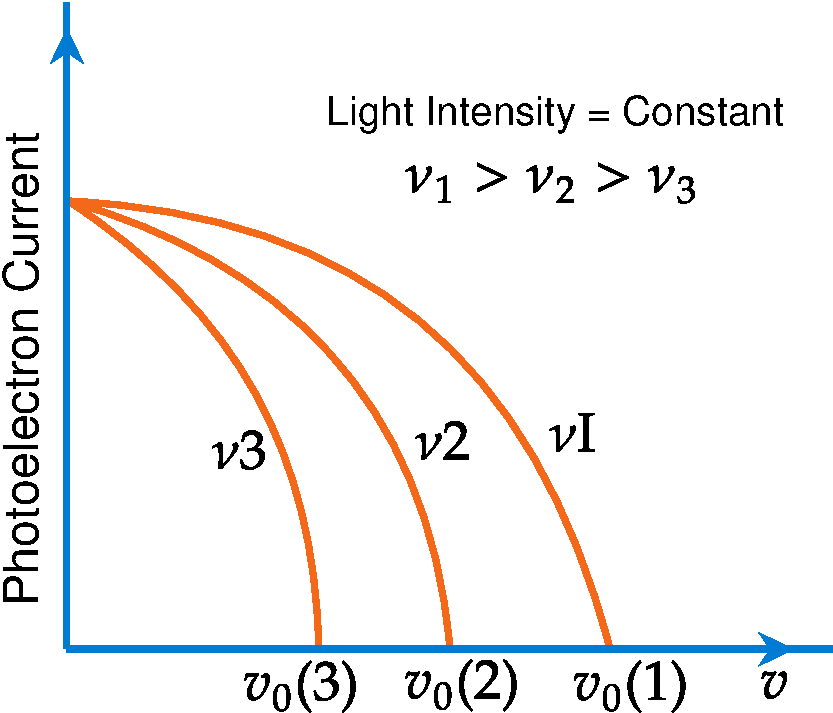
\includegraphics[height=4.5cm,width=5cm]{7-crop}
	\caption{}
	\label{photo3}
\end{figure} 
Here, \   $\nu_1>\nu_2>\nu_3 \rightarrow KE_1>KE_2>KE_3 \ \rightarrow v_0(1)>v_0(2)>v_0(3)$

\subsubsection{Einstein's Photoelectric Equation }
According to Einstein's explanation, photoelectric effect occurs due to absorption of a single photon by an electron in the atom. When radiation falls on a metal surface, an electron may absorb one quantum of energy and increase its energy by $h \nu $.  Some of the absorbed energy, $\phi$, will be used to separate the electron from the metal surface. The surplus energy appears as the kinetic energy of the emitted electron.
$$
K . E .=h \nu-\phi
$$
The electrons which are more tightly bound to the metal (e.g. electrons which lie two or three atomic layers below the surface) require more energy to be removed. We define \textbf{Work Function} $\phi$ of a metal as the
minimu energy that must be supplied to an electron at the metal surface to dislodge it from the metal.  Such electrons are emitted with maximum possible kinetic energy. Thus Einstein's equation becomes,
$$
KE_{\max }=\frac{1}{2} m v_{\max }^{2}=h \nu-\phi
$$
Since kinetic energy cannot be negative, the above equation implies the existence of a minimum frequency $\nu_{0}$ for photoemission to take place
$$
h \nu_{0}=\phi \quad \Rightarrow {\nu }_{0}=\frac{\phi}{h}
$$
Using this, we can  rewrite Einstein's equation as,
$$
KE_{\max }=h\left(\nu-\nu_{0}\right)
$$
\textbf{Work Function:}\\\\
The minimum energy $\phi$ of an electron to escape from a particular metal surface is called work function of the metal 
$$\phi=h\nu_0$$
Where $v_0$ is the critical frequency below which no photoelectrons are emitted. The greater the work function of a metal, the more energy is needed for an electron to leave it's surface, and the higher the critical frequency for photo electric emission to occur.
\begin{exercise}
	The minimum frequency for photo electric emission in copper is $1.1\times10^{15} Hz$ \ Find the maximum energy of the photoelectron (electron volts)when light of frequency $1.5\times10^{15} Hz$\  is directed on a copper surface.
\end{exercise}
\begin{answer}
	\begin{align*}
	KE_{max}&=h(\nu-\nu_0)\\
	\nu&=1.5\times10^{15} Hz\\
	\nu_0&=1.1\times10^{15} Hz\\
	KE_{max}&=6.6\times10^-34(1.5\times10^{15}-1.1\times10^{15})\\
	&=6.6\times10^-34\times0.4\times10^{15}\\
	&=2.64\times10^{-19} J\\
	KE_{max}&=\frac{2.64\times10^{-19}}{1.6\times10^{-19}}\\
	&=1.65ev
	\end{align*}
\end{answer}
\subsection{X-rays and Compton effect.}
X-rays were discovered accidentally by German scientist Rontgen in 1895. The first Nobel Prize was awarded to Rontgen in 1901. Within a few years it became clear that x-rays are another form of electromagnetic radiation of wavelengths typically some tens or hundreds of picometers (1 $\mathrm{pm}=10^{\wedge}-12 \mathrm{~m}$ ). These are  highly penetrating electromagnetic radiation and it has proved to be a very powerful tool to study the crystal structure, in material research and in various other fields of science and technology.  X-rays are highly energetic radiations with very short wavelengths.
\subsubsection{Properties}
\begin{itemize}
	
	\item  X-rays do not require any medium for propagation and they cannot be refracted.
	\item  Electric and magnetic fields do not have any effect on these rays.
	\item  These radiations ionize the surrounding air by discharging electrified bodies.
	\item   X-rays have short wavelength varying between $0.1 $ \AA \ to $1 $\AA.
	\item   X-rays are produced when a metal anode is bombarded by very high energy electrons.
\end{itemize}
\subsubsection{X-ray - Diffraction.}
$X$ - ray diffraction is one of the earliest methods for studying the structure of solids. In the process of diffraction, electromagnetic waves of a given frequency but different phases interact to produce constructive interference (bright spots on the film exposed to the light) and destructive interference (dark spots). By a careful analysis of the diffraction patterns, very accurate values of the lattice parameters (unit cell dimensions) can be inferred.
The $x$ -rays only for a particular angle of incidence, such that x-ray beams reflected from successive planes of atoms have their electric and magnetic fields in phase.
The atomic planes of a crystal cause an incident beam of X-rays to interfere with one another as they leave the crystal. The phenomenon is called X-ray diffraction. Diffraction occurs only when Bragg's Law is satisfied the condition for constructive interference  from planes with spacing ${d}$.
\subsubsection{Bragg's law}
Bragg's  law plays a central role in  the analysis of diffraction data. This law relates the angle $\theta$ ( at which there is a maximum in diffracted intensity ) to the wavelength $\lambda$ of $X$ -rays and the inter-layer distance $\mathrm{d}$ between the planes of atoms , ions or molecules in the lattice. 
Mathematically the condition can be  written as,
\begin{equation}
2 d \sin \theta=n \lambda \quad n=1,2,3, \ldots
\qquad \text{Bragg'ss law.}
\end{equation}

\subsection{Compton Effect}
Photoelectric effect provides evidence that energy is quantized. In order to establish the particle nature of radiation, it is necessary that photons must carry momentum.  In 1922, Arthur Compton studied the scattering of $x$ -rays of known frequency from graphite and looked at the recoil electrons and the scattered $x$ -rays.The hypothesis proposed by Arthur Compton  suggested that when an X-ray quantum is scattered it spends all of its energy and momentum upon some particular electron. This electron in turn scatters the ray in some definite direction. The change in momentum of the X-ray quantum due to the change in its direction of propagation results in a recoil of the scattering electron. The energy in the scattered quantum is thus less than the energy in the primary quantum by the kinetic energy of the recoil of the electron.
\begin{figure}[H]
	\centering
	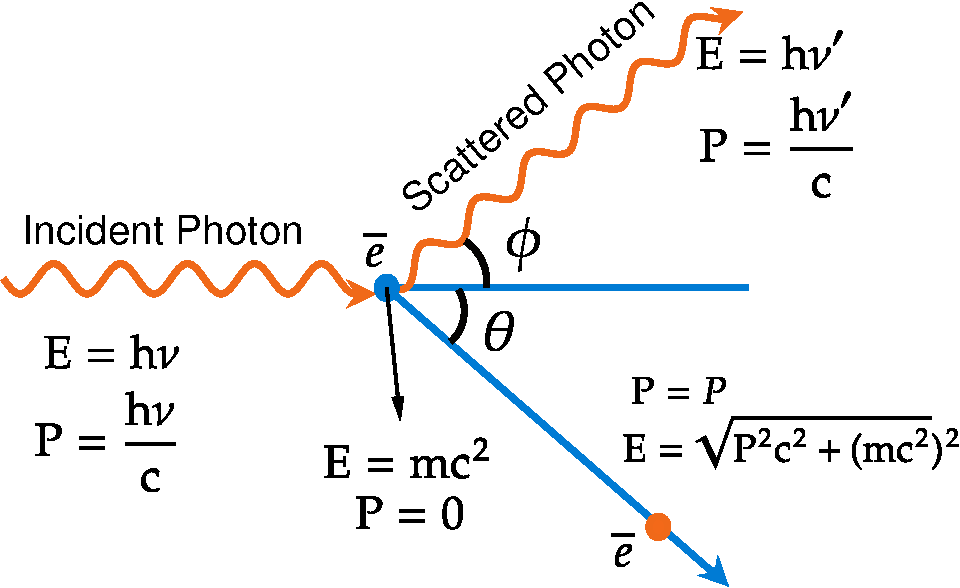
\includegraphics[height=5cm,width=7.5cm]{9-crop}
	\caption{Compton effect}
	\label{}
\end{figure}
\begin{align*}
h\nu&=\quad \text{The energy of incident photon}\\
\frac{h\nu}{c}&=\quad \text{Momentum of incident photon}\quad [E=Pc \therefore P=\frac{E}{c}]\\
h\nu\prime&=\quad\text{The energy of scattered photon}\\
\frac{h\nu\prime}{c}&=\quad \text{Momentum of scattered photon}\\
h\nu&>h\nu\prime\\
KE \text{ of electron }&=h\nu-h\nu\prime\\
E&=\quad mc^2 \ \text{is the rest energy of electrons. }\\
E&=\sqrt{P^2c^2+(mc^2)^2}\text{ is the total energy of scattered electron.}\\
\phi&=\text{ The scattering angle for incident photon.}\\
\theta&= \text{ The angle between the direction of initial photon and the recoil electron.}
\end{align*}
If we treat the incident radiation as a stream of particles which are named as photons-colliding elastically with individual electrons.  In that scattering process we use the laws of elastic collisions the conservation of energy and momentum.\\
\begin{figure}[H]
	\centering
	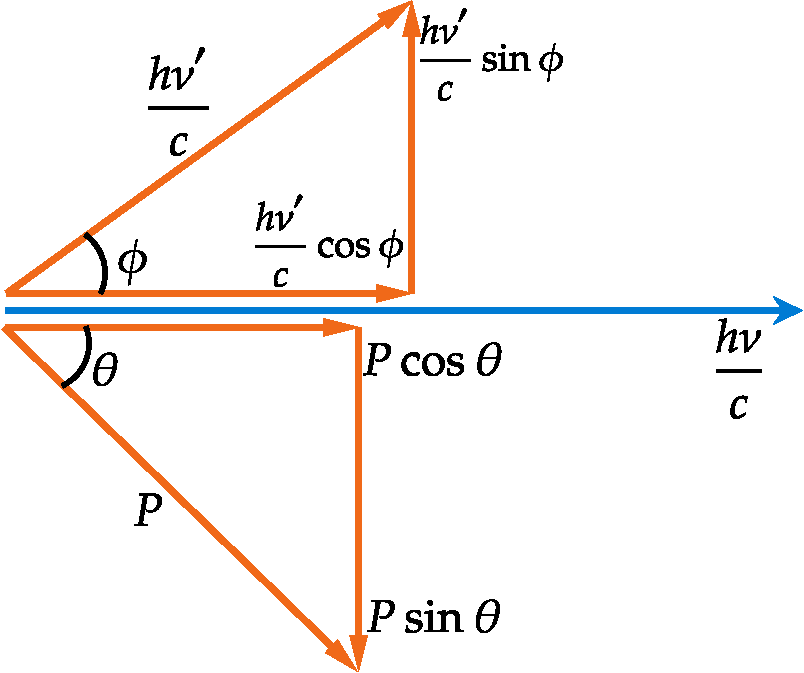
\includegraphics[height=6cm,width=7cm]{13-crop}
	\caption{}
	\label{}
\end{figure}



\begin{align}
\intertext{By using momentum conservation,}\notag
\text { Initial momentum }&=\text { final momentum } \\
\qquad \frac{h \nu}{c}+0&=\frac{h \nu^{\prime}}{c} \cos \phi+p \cos \theta\\
pc\cos\theta&=h\nu-h\nu^\prime\cos\phi \label{comp1}
\intertext{In perpendicular to this direction,}
0&=\frac{h \nu^{\prime}}{c} \sin \phi-p \sin \theta\\\label{comp2}
pc\sin\theta&=h\nu^\prime\sin\phi
\intertext{By squaring  equations \ref{comp1} and \ref{comp2} and adding the new ones together, the angle $\theta$ is eliminated, leaving}
p^{2} c^{2}&=(h \nu)^{2}-2(h \nu)\left(h \nu^{\prime}\right) \cos \phi+\left(h \nu^{\prime}\right)^{2}\label{comp3}
\intertext{The total energy of scattered particle can be written as,}
E&=\mathrm{KE}+m c^{2} \qquad \text{And} \qquad
E=\sqrt{m^{2} c^{4}+p^{2} c^{2}} \intertext{Equating both of them we get,}
\left(\mathrm{KE}+m c^{2}\right)^{2}&=m^{2} c^{4}+p^{2} c^{2} \\
p^{2} c^{2}&=\mathrm{KE}^{2}+2 m c^{2} \mathrm{KE}\\
\because \mathrm{KE}=h \nu-h \nu^{\prime}\\
p^{2} c^{2}&=(h \nu)^{2}-2(h \nu)\left(h \nu^{\prime}\right)+\left(h \nu^{\prime}\right)^{2}+2 m c^{2}\left(h \nu-h \nu^{\prime}\right) 
\intertext{Substituting the value of $P^2c^2$ in equation. \ref{comp3}  , we get}
2 m c^{2}\left(h \nu-h \nu^{\prime}\right)&=2(h \nu)\left(h \nu^{\prime}\right)(1-\cos \phi)\label{comp4}
\intertext{In terms of wavelength, equation. \ref{comp4} \ becomes,}
\frac{m c}{h}\left(\frac{\nu}{c}-\frac{\nu^{\prime}}{c}\right)&=\frac{\nu}{c} \frac{\nu^{\prime}}{c}(1-\cos \phi)
\intertext{And so, since $v / c=1 / \lambda$ and $\nu^{\prime} / c=1 / \lambda^{\prime}$,}
\frac{m c}{h}\left(\frac{1}{\lambda}-\frac{1}{\lambda^{\prime}}\right) &=\frac{1-\cos \phi}{\lambda \lambda^{\prime}} \\
\lambda^{\prime}-\lambda &=\frac{h}{m c}(1-\cos \phi)\label{comp5}
\intertext{Equation \ref{comp5} gives the change in wavelength expected for a photon that is scattered through the angle $\phi$ by a particle of rest mass $m$. This change is independent of the wavelength $\lambda$ of the incident photon. }\notag
\end{align}
\begin{center}
	\framebox{
		\parbox[t][1cm]{5cm}{
			
			\addvspace{0.3cm} \centering
			
			
			$\Delta\lambda=\lambda^\prime-\lambda=\lambda_c\left( 1-\cos\phi\right)$ 
	} }
\end{center}

\begin{align*}
\lambda_c&=\frac{h}{mc}
\intertext{$\lambda_c$ is called Compton wavelength of the scattered particle. For electron }
\lambda_c&=2.426\times10^{-12}m\\
\lambda_c&=2.426 \text{pm}
\end{align*}
\begin{note}
	\textbf{1)}\quad The shift is independent of the wavelength $\lambda$ of incident photon. Which depends only on the scattering angle$\phi$, and the constant parameters $h,c$ and mass of the particle scattered.\\
	
	\textbf{2)}\quad The shift is maximum when $\phi=180$ ie when it scattered back in the incident direction.\\
	\textbf{3)}\quad The maximum $KE$ of the recoil electron occure when $\phi=180$
	$$KE_{max}=\frac{2h^2\nu^2}{mc^2}\frac{1}{\left(1+\frac{2h\nu}{mc^2} \right) }$$
\end{note}
\begin{exercise}
	How much energy muct a photon have . If it is to have the momentum of a $10Mev$\ proton.
\end{exercise}
\begin{answer}
	\begin{align*}
	KE&=\frac{P^2}{2m}\\
	P&=\sqrt{2mkE}\\
	&=\sqrt{2\times1.67\times10^{-27}\times10\times10^6\times1.6\times10^{-19}}\\
	&=7.31\times10^{-20}kg m/s\\
	\text{For photon }E&=Pc\\
	E&=7.31\times10^{-20}\times3\times10^8\\
	E&=21.93\times10^{-12} J\\
	E&=\frac{21.93\times10^12}{1.6\times10^{-19}}ev\\
	&=13.706\times10^7\\
	&=137 Mev
	\end{align*}
\end{answer}
\begin{exercise}
	A monochromatic X-ray beam whose wavelength is $55.8pm$ is scattered through $46^\circ$. Find the wavelength of the scattered beam.
\end{exercise}
\begin{answer}
	\begin{align*}
	\lambda\prime -\lambda&=\lambda_c(1-\cos\phi)\\
	\lambda&=55.8\times10^{-12}m\\
	\lambda_c&=2.426\times10^{-12}m\\
	\phi&=46^\circ\\
	\lambda\prime&=\lambda+\lambda_c(1-\cos\phi)\\
	&=55.8pm+0.742 pm\\
	&=56.54 pm
	\end{align*}
\end{answer}
\subsection{Pair production}
Unlike Photoelectric effect and Compton effect,  the photon, passing near the nucleus of an atom,  subjected to strong field effects from the nucleus  may disappear as a photon and reappear as a positive and negative electron pair. This process is called the pair production. In  pair production,  electromagnetic energy is converted into matter.  No conservation principles are violated when an electron positron pair is created.\\
the photon must have a minimum energy to pair production take place,
The rest energy $m c^{2}$ of an electron or positron is $0.51 \mathrm{MeV}$, hence pair production requires a photon energy of at least $1.02 \mathrm{MeV}$. Any additional photon energy becomes kinetic energy of the electron and positron. The corresponding maximum photon wavelength is $1.2 \mathrm{pm}$. Electromagnetic waves with such wavelengths are called gamma rays, symbol $\gamma$, and are found in nature as one of the emissions from radioactive nuclei and in cosmic rays. \\
The kinetic energy of the electrons produced will be the difference between the energy of the incoming photon and the energy equivalent of two electron masses (  $1.022 \mathrm{MeV})$.
$$
{E}_{{e}+}+{E}_{{e}-}={h} v-{1 . 0 2 2}({M e V})
$$
The inverse of pair production occurs when a positron is near an electron and the two come together under the influence of their opposite electric charges. Both particles vanish simultaneously, with the lost mass becoming energy in the form of two gamma-ray photons:
$$
e^{+}+e^{-} \rightarrow \gamma+\gamma
$$
And this process is called pair annihilation.
\section{WAVE ASPECTS OF PARTICLES}
\subsection{de Broglie's hypothesis:matter waves}
As discussed above-in the photoelectric effect, the Compton effect, and the pair production effect-radiation exhibits particle-like characteristics in addition to its wave nature. In 1923 de Broglie took things even further by suggesting that this wave-particle duality is not restricted to radiation, but must be universal: all material particles should also display a dual wave-particle behavior. That is, the wave-particle duality present in light must also occur in matter.\\
So, starting from the momentum of a photon $p=h \nu / c=h / \lambda$, we can generalize this relation to any material particle  with nonzero rest mass: each material particle of momentum $\vec{p}$ behaves as a group of waves (matter waves) whose wavelength $\lambda$ and wave vector $\vec{k}$ are governed by the speed and mass of the particle\\
$$\lambda=\frac{h}{p}, \quad \vec{k}=\frac{\vec{p}}{\hbar}$$
where $\hbar=h / 2 \pi$. The expression known as the de Broglie relation, connects the momentum of a particle with the wavelength and wave vector of the wave corresponding to this particle.\\
\begin{exercise}
	Calculate the wavelength associated with a cricket ball of mass $0.2 \mathrm{~kg}$ moving with a speed of $30 \mathrm{~m} / \mathrm{s}$.
\end{exercise}
\begin{answer}
	\begin{align*}
	p&=m v=0.2 \times 30\\&=6 \mathrm{~kg} \mathrm{~m} / \mathrm{s} \\
	\lambda&=\frac{h}{p}\\&=\frac{6.63 \times 10^{-34}}{6}\\&=1.1 \times 10^{-34} \mathrm{~m}
	\end{align*}
\end{answer}
\begin{exercise}
	What is the speed of an electron if its de Broglie wavelength equals its Compton wavelength ?
\end{exercise}
\begin{answer}
	\begin{align*}
	\lambda_{Rel}&=\frac{h}{p}=\frac{hc}{pc}\\
	&=\frac{hc}{\sqrt{E^{2}-E_{0}^{2}}}\hspace{4cm}\text{But} \ E=\gamma E_{0}\\
	&=\frac{hc}{\sqrt{\gamma E_{0}^{2}-E_{0}^{2}}}
	=\frac{hc}{\sqrt{E_{0}^{2}(\gamma ^{2}-1)}}\\
	&=\frac{hc}{ m_{0} c\sqrt{(\gamma ^{2}-1)}}=\frac{hc}{ m_{0} c^{2}\sqrt{(\gamma ^{2}-1)}}\\
	&=\frac{\lambda_{C}}{ \sqrt{(\gamma ^{2}-1)}}\hspace{4.5cm} \gamma=\sqrt{1-\frac{v^{2}}{c^{2}}}
	\intertext{Then if de Broglei wavelength equals Compton wavelength then,}
	\lambda_{Rel}&=\lambda_{C}\\
	1&=\frac{1}{ \sqrt{(\gamma ^{2}-1)}}\\
	\gamma ^{2}&=2 \Rightarrow \gamma= \sqrt{2}\\
	\sqrt{2}&=\frac{1}{\sqrt{1-\frac{v^{2}}{c^{2}}}}\\
	\text{On solving we get,}\ v&=\frac{c  }{\sqrt{2}}.
	\end{align*}
\end{answer}
\subsection{Velocity of a Matterwave}\label{velocity of matter wave}
We know that every material paticle in motion is assoiated with a wave called matterwave. 
\begin{align}
\intertext{According to the mass energy relation,}
E&=mc^{2}\\
\text{For a matterwave,}\ E&=h\nu\\
\text{Then,}\ h\nu&=mc^{2} \Rightarrow
\nu=\frac{mc^{2}}{h}\\
\text{Velocity of a wave,}\ v&=\nu\lambda\\
v_{mw}&=\frac{mc^{2}}{h} \times \frac{h}{mv} \hspace{2cm} \lambda=\frac{h}{p}=\frac{h}{mv}\\
v_{mw}&=\frac{c^{2}}{v}>>>c
\end{align}
That is the velocity of de-Broglei wave associated with a moving material is greater than the velocity of light. But according to the special theory of relativity, no energy can be transmitted with velocity greater than $\mathrm{c}$. So we need  to explain the behaviour of matterwave. 

\subsection{Phase velocity}
The phase velocity \ $v_{p}$\ of a wave is the rate at which the phase of the wave propagates in space. It is also the velocity of a monochromatic wave with which crest or trough of the wave travels in a medium.
A plane wave propogating along the $ +{ve} $\ x-direction can be represented as,
\begin{align}
\psi(x,t)&=A\ e^{i(kx-\omega t)}\\ \notag
\omega&= \text{The angular frequency.}\\ \notag v&= \text{The velocity.}\\\notag A&=\text{ The amplitude of the wave.}
\intertext{The phase $\phi$ of the wave at any time ' $t$ ' at a distance ' $x$ ' from the origin is ,}
\phi(x, t)&=(k x-\omega t)
\intertext{We know that the phase of a wave is a constant quantity, then,}
k x-\omega t&= \text{constant}\\
k dx-\omega dt&=0\\
\notag k dx&=\omega dt\\
\frac{dx}{dt}&=\frac{\omega}{k}\\
v_{p}&=\frac{\omega}{k}
\intertext{Multiplying numerator and denominator by \ $\hbar$\ we get,}
v_{p}&=\frac{\hbar\omega}{\hbar k}\\
v_{p}&=\frac{E}{p} \hspace{2cm} \text{Since,}\quad E=\hbar\omega \ \text{and}\ p=\hbar k
\end{align}
\begin{center}
	\framebox{
		
		\parbox[t][1.5cm]{4cm}{
			
			\addvspace{0.2cm} \centering
			\textbf{Phase velocity}\\\vspace{0.2cm} 
			$v_{p}=\frac{\omega}{k} \quad;\quad v_{p}=\frac{E}{p}$} 
	}
\end{center}
The phase velocity  of a matter wave can be obtained as,
\begin{align}
\intertext { From the relativistic mass energy relation, } {v}_{p}&=\frac{E}{p}\\&=\frac{\gamma m_{0} c^{2}}{\gamma m_{0} v} \hspace{1cm} m_{0}= \text{Rest mass of the particle}\quad ; \quad \gamma=\frac{1}{\sqrt{1-\frac{v^{2}}{c^{2}}}}\\{v}_{p}&=\frac{c^{2}}{v}
\end{align}
The phase velocity of a de-Broglie wave is always greater than the velocity of light in freespace. But according to the special theory of relaticvity, no energy can be transmitted with velocity greater than $ c $. This suggests that the phase velocity has no physical significance and we can not respresent the wave nature of a moving particle by a single plane wave. Thus what we have derived in section.\ref{velocity of matter wave} is the phase velocity of the matterwave.
\subsection{Group velocity}
A moving particle is not associated with a single wave but a group of waves called wavepacket.
A wave packet therefore consists of a
group of waves of slightly different wavelengths, with phases and amplitudes so chosen that
they interfere constructively over a small region of space and destructively elsewhere.
Let, the wave group is formed by the superposition of two monochromatic waves having same amplitude but differing in angular frequency by an amount ' $\Delta \omega$ ' and in wave number ' $\Delta k$ ' i.e
$$
\begin{array}{l}
\psi_{1}(x,t)=A \sin (\omega t-k x) \\
\psi_{2}(x,t)=A \sin [(\omega+\Delta \omega) t-(k+\Delta k) x]
\end{array}
$$
The resultant wave i.e. wave packet can be written as,
$$
\psi(x,t)=2 A \cos \left[\frac{1}{2}(\Delta \omega t-\Delta k x)\right] \sin (\omega t-k x)
$$
Now, group velocity is the velocity with which maximum amplitude or the envelope of the wave packet moves and it is given as: $$v_{g}=\frac{d \omega}{d k}=\frac{d E}{d p}$$.
From the relativistic mass-energy relation :


\begin{align}
E^{2}&=p^{2} c^{2}+m_{0}^{2} c^{4} \quad \Rightarrow 2 E \frac{d E}{d p}=2 p c^{2} \\
v_{g}&=\frac{d E}{d p}=\frac{p c^{2}}{E}\\&=\frac{\gamma m_{0} v c^{2}}{\gamma m_{0} c^{2}}\\v_{g}&=v <c
\end{align}
\begin{center}
	\framebox{
		
		\parbox[t][1.5cm]{4cm}{
			
			\addvspace{0.2cm} \centering
			\textbf{Group velocity}\\\vspace{0.2cm} 
			$v_{g}=\frac{d\omega}{dk} \quad;\quad v_{g}=\frac{dE}{dp}$} 
	}
\end{center}
\begin{note} \hspace{0.6cm}
	\textbf{\large Other useful expressions for Group velocity}\\
	\begin{minipage}{0.30\textwidth}
		\begin{align*}
		v_{g}&=\frac{d\omega}{dk}\\
		&=\frac{d (\hbar\omega)}{d (\hbar k) }\\
		&= \frac{1}{ \hbar }\frac{d (\hbar\omega)}{dk}\\
		v_{g}&= \frac{1}{ \hbar }\frac{d E}{d   k}
		\end{align*}
	\end{minipage}
	\begin{minipage}{0.30\textwidth}
		\begin{align*}
		v_{g}&=\frac{d\omega}{dk}\\
		&=\frac{d (2 \pi \nu)}{d (2\pi/\lambda) }\\
		&= \frac{ 2 \pi }{ 2\pi }\cdot \frac{d (2 \pi \nu)}{d (2\pi/\lambda) }\\
		v_{g}&= \frac{-1}{ \lambda^{2} }\frac{d \nu}{d \lambda}
		\end{align*}
	\end{minipage}
\end{note}
\subsection{Group and Phase Velocities}

When we superimpose many waves of different amplitudes and frequencies, we can obtain a wave packet or pulse which travels at the group velocity $v_{g}$; the individual waves that constitute the packet, however, move with different speeds; each wave moves with its own phase velocity $v_{p h}$. Figure .\ref{phase and group velocity} gives a qualitative illustration: the group velocity represents the velocity with
which the wave packet propagates as a whole, where the individual waves (located inside the
packet’s envelope) that add up to make the packet move with different phase velocities.
\begin{figure}[H]
	\centering
	\includegraphics[height=4cm,width=6cm]{phase and group velocity }
	\caption{Phase and group velocity}
	\label{phase and group velocity}
\end{figure}
\subsection{de-Broglei's Dispersion relation}
The dispersion relation for de Broglie waves 
\begin{align}
v_{p}&=\frac{\omega}{k}\ \qquad \text{And}\qquad v_{g}=\frac{d\omega}{dk}\\
V_{g} &=\frac{d}{d k}\left(v_{p} k\right) 
=v_{p}\cdot 1+ k \frac{d v_{p}}{d k} \notag \\
&=v_{p}+k \frac{d v_{p}}{d{k}} \hspace{5cm}  \begin{array}{ll}
k&=\frac{2 \pi}{\lambda}\\
dk&=\frac{-2 \pi}{\lambda^{2}} d\lambda
\end{array}  \\
&=v_{p}+\frac{2 \pi}{\lambda}  d v_{p}\ \cdot \frac{-\lambda^{2}}{2 \pi d \lambda} \notag \\
v_{g} &=v_{p}-\lambda \frac{d v_{p}}{d \lambda}  \qquad\rightarrow (\text{Dispersion relaion.})
\end{align}
\begin{center}
	\framebox{
		
		\parbox[t][2.0cm]{4cm}{
			
			\addvspace{0.2cm} \centering 
			$\begin{array}{ll}
			v_{g}&=v_{p}+k \frac{d v_{p}}{d{k}}\\\\
			v_{g} &=v_{p}-\lambda \frac{d v_{p}}{d \lambda}
			\end{array}$
			
		} 
	}
\end{center}
Dispersive medium are of two types:
\begin{itemize}
	\item  Normal dispersive medium: $\frac{d v_{p}}{d \lambda}=+v e \Rightarrow v_{g}<v_{p}$.
	\item  Anamolous dispersive medium: $\frac{d v_{p}}{d \lambda}=-v e\Rightarrow v_{g}>v_{p}$.
\end{itemize}
For, non-dispersive medium, all waves travel with same phase velocity: $\frac{d v_{p}}{d \lambda}=0 \Rightarrow v_{g}=v_{p}$.
\subsection{ Phase and group velocity Relation  for a free particle}
For a free particle the potential energy is zero . Then,
\begin{align}
E&=\text{K.E}= \frac{p^{2}}{2m} \label{freeparticle 1}\\
v_{p} &=\frac{E}{p} \label{freeparticle 2}
\intertext{Puttting  equation. \ref{freeparticle 1} in \ref{freeparticle 2} , we get,}
v_{p} &=\frac{p}{2m}\notag\\
v_{g} &=\frac{d E}{d p} \\
&=\frac{2p}{2m}=\frac{p}{m} \\
v_{g} &=2V_{p}
\end{align}
\begin{center}
	\framebox{
		
		\parbox[t][1.5cm]{4cm}{
			
			\addvspace{0.2cm} \centering 
			\textbf{Free particle}\\\vspace{0.2cm} 
			$v_{g} =2v_{p}$} 
	}
\end{center}
\subsection{ Phase and group velocity Relation  for a relativistic particle}
For a relativistic particle, The energy \ $E$\ is given by,
\begin{align}
E^{2} &=p^{2} c^{2}+m_{0}^{2} c^{4} \\
E &=\sqrt{p^{2} c^{2}+m_{0}^{2} c^{4}}\notag \\
v_{p} &=\frac{E}{p} \\
&=\sqrt{\frac{p^{2} c^{2}+m_{0}^{2} c^{4}}{p^{2}}}\notag \\
v_{g} &=\frac{d E}{d p} \\
&=\frac{{2 p c^{2}}}{2 \sqrt{p^{2} c^{2}+m_{0}^{2} c^{4}}}\notag \\
&=\frac{p c^{2}}{\sqrt{p^{2} c^{2}+m_{0}^{2} c^{4}}} . \\
v_{p} \cdot v_{g}&=\sqrt{\frac{p^{2} c^{2}+m_{0}^{2} c^{4}}{p^{2}}}\cdot \frac{p c^{2}}{\sqrt{p^{2} c^{2}+m_{0}^{2} c^{4}}}\\
v_{p} \cdot v_{g}&=c^{2}
\end{align}
\begin{center}
	\framebox{
		
		\parbox[t][1.5cm]{4cm}{
			
			\addvspace{0.2cm} \centering 
			\textbf{Relativistic particle}\\\vspace{0.2cm} 
			$v_{p} \cdot v_{g}=c^{2}$} 
	}
\end{center}
\begin{minipage}{0.25\textwidth}
	\colorlet{ocre1}{ocre!70!}
	\colorlet{ocrel}{ocre!30!}
	\begin{table}[H]
		\centering
		\arrayrulecolor{ocre}
		\renewcommand{\arraystretch}{2.5}
		\begin{tabularx}{1\textwidth} { 
				| >{\centering\arraybackslash}X 
				|   }
			\hline
			\rowcolor{ocrel} \large \textbf{Phase Velocity $v_{p}$} \\
			\hline
			\hline
			$\begin{array}{l}
			v_{p} =\frac{\omega}{k} \\
			v_{p} =\frac{E}{p}\\
			\end{array}$\\ \hline
			
			
		\end{tabularx}
		
	\end{table}
\end{minipage}
\begin{minipage}{0.25\textwidth}
	\colorlet{ocre1}{ocre!70!}
	\colorlet{ocrel}{ocre!30!}
	\begin{table}[H]
		\centering
		\arrayrulecolor{ocre}
		\renewcommand{\arraystretch}{2.5}
		\begin{tabularx}{1\textwidth} { 
				| >{\centering\arraybackslash}X 
				|   }
			\hline
			\rowcolor{ocrel} \large \textbf{Group Velocity $v_{g}$} \\
			\hline
			\hline
			$\begin{array}{l}
			v_{g} =\frac{d\omega}{dk} \\
			v_{g} =\frac{dE}{dp}\\
			v_{g}= \frac{1}{ \hbar }\frac{d E}{d   k}\\
			v_{g}= \frac{-1}{ \lambda^{2} }\frac{d \nu}{d \lambda}
			\end{array}$\\ \hline
			
			
		\end{tabularx}
		
	\end{table}
\end{minipage}
\begin{minipage}{0.40\textwidth}
	\colorlet{ocre1}{ocre!70!}
	\colorlet{ocrel}{ocre!30!}
	\begin{table}[H]
		\centering
		\arrayrulecolor{ocre}
		\renewcommand{\arraystretch}{2.5}
		\begin{tabularx}{1\textwidth} { 
				| >{\centering\arraybackslash}X 
				|   }
			\hline
			\rowcolor{ocrel} \large \textbf{Relation between $v_{p}$ and $v_{g}$} \\
			\hline
			\hline
			$\begin{array}{l}
			v_{g}=v_{p}+k \frac{d v_{p}}{d{k}}\\
			v_{g} =v_{p}-\lambda \frac{d v_{p}}{d \lambda} \\
			v_{g} =2v_{p}\quad \rightarrow\text{Free particle} \\
			v_{p} \cdot v_{g}=c^{2}\rightarrow\text{Relativistic particle}
			\end{array}$\\ \hline
			
			
		\end{tabularx}
		
	\end{table}
\end{minipage}
\section{The Wave equation}
The wave equation governs many physical phenomenon in nature. It is important to  understand the properties of wave propogation. Here we are discussing the one dimensional wave equation, like the one in a stretched string. The results are however readily transferable or modified for sound waves any and other types of waves.
The standared form of wave equation is ,
\begin{equation}\label{wave eq1}
\frac{\partial^{2} y}{\partial x^{2}}=\frac{1}{v^{2}} \frac{\partial^{2} y}{\partial t^{2}}
\end{equation}
\begin{figure}[H]
	\centering
	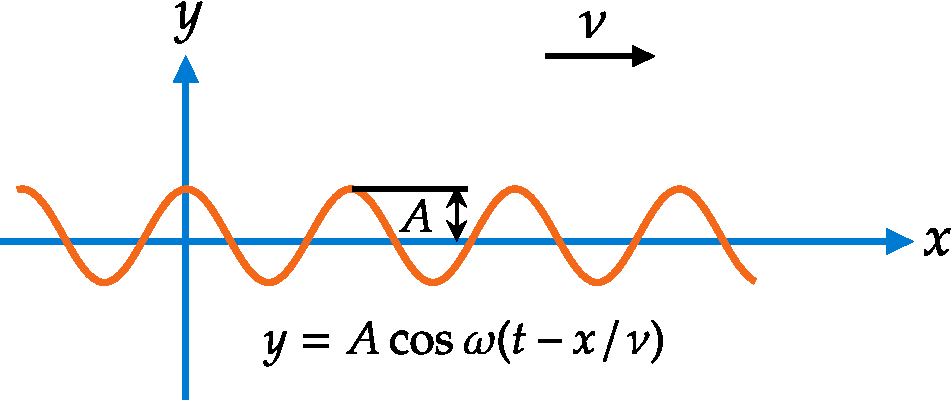
\includegraphics[height=3cm,width=5cm]{quantum wave1}
	\caption{Waves in the $x y$ plane traveling in the $+x$ direction }
	\label{quantum wave1}
\end{figure}
where, it's  a wave whose variable quantity is $y$ that propagates in the $x$ direction with the speed $v$. In the case of a wave in a stretched string, $y$ is the displacement of the string from the $x$ axis; in the case of a sound wave, $y$ is the pressure difference. The properties of wave propogation is derived from the solutions of the wave equation . The soultion is obtained by the method of seperation of variables. All solutions must be of the form,
\begin{equation}\label{wave eq2}
y=F\left(t \pm \frac{x}{v}\right)
\end{equation}
Where $ F $ is any function that can be differentiated. The solutions $F(t-\frac{x}{v})$ represent waves traveling in the $+x$ direction, and the solutions $F(t+\frac{x}{v})$ represent waves traveling in the $-x$ direction. 
The wave equivalent of a "free particle," which is a particle that is not under the influence of any forces and therefore pursues a straight path at constant speed. This wave is described by the general solution of Equation.\ref*{wave eq1} for undamped (constant amplitude $ A $), monochromatic (constant angular frequency $\omega$ ) harmonic waves in the $+x$ direction. The solution is of the form,
\begin{equation}\label{wave eq3}
y=A e^{-i \omega(t-x / v)}
\end{equation}
\begin{equation}\label{wave eq4}
y=A \cos \omega\left(t-\frac{x}{v}\right)-i A \sin \omega\left(t-\frac{x}{v}\right)
\end{equation}

\section{Schrödinger equation: Time-dependant form}
It was observed that the wave function of a particle of fixed energy $ E$ could  be written as a linear combination of wave functions of the form,
\begin{equation}\label{schro 1}
\psi=A e^{-i \omega(t-x / v)}
\end{equation}
The above equation.\ref*{schro 1}, represents  a wave travelling in the positive $ x $ direction.The physical quantity,  $\psi$ is the 'wave function' corresponds to the wave variable $y$ of wave motion in general. 
\begin{align}
\text{We know that,}
\omega&=2 \pi \nu \\
v&=\lambda \nu
\intertext{Replacing $\omega$  and $v$ in the above formula  we get, }
\psi&=A e^{-2 \pi i(\nu t-x / \lambda)}
\intertext{But we know that,}
E&=h \nu=2 \pi \hbar \nu \quad \text { Since,}\ \hbar=\frac{h}{2\pi}  \\\text { And } \quad \lambda&=\frac{h}{p}=\frac{2 \pi \hbar}{p}
\intertext{Then the solution of the free particle becomes,}
\psi&=A e^{-(i / \hbar)(E t-p x)}\label{schro2}
\intertext{The Schrödinger equation is not a one which can be derived from any basic principles, since  itself  the Schrödinger equation is a basic principle. But we  can be arrived at the equation in various ways. Differentiating  the equation . \ref*{schro2} twice with respect to $x$, we get,}
\frac{\partial^{2} \psi}{\partial x^{2}} &=-\frac{p^{2}}{\hbar^{2}} \psi \label{schro4} \\
p^{2} \psi &=-\hbar^{2} \frac{\partial^{2} \psi}{\partial x^{2}}
\intertext{ Differentiating  the equation . \ref*{schro2} twice with respect to $t$, we get,}
\frac{\partial \psi}{\partial t} &=-\frac{i E}{\hbar} \psi \\
E \psi &=-\frac{\hbar}{i} \frac{\partial \psi}{\partial t}\label{schro5}
\intertext{A particle of mass ' $\mathrm{m}$ '  moving along $x$ axis, under the potential field $V(x)$ which is independent of time. The total energy of the system can be written as,}
E&=E_{k}+E_{p}=\frac{p_{x}^{2}}{2 m}+V(x,t)\label{schro3}
\intertext{Multiplying both sides of Equation. \ref*{schro3} by the wave function $\psi$ gives,}
E \psi&=\frac{{p(x)}^{2} \psi}{2 m}+V(x,t) \psi
\intertext{Substituting for $E \psi$ and $p^{2} \psi$ from Equations.\ref{schro4} and \ref{schro5} to obtain the time-dependent form of Schrödinger's equation,}
i \hbar \frac{\partial \psi}{\partial t}&=-\frac{\hbar^{2}}{2 m} \frac{\partial^{2} \psi}{\partial x^{2}}+V(x,t) \psi
\intertext{In 3-D, the Schrödinger's equation becomes,}
i \hbar \frac{\partial \psi}{\partial t}&=-\frac{\hbar^{2}}{2 m}\left(\frac{\partial^{2} \psi}{\partial x^{2}}+\frac{\partial^{2} \psi}{\partial y^{2}}+\frac{\partial^{2} \psi}{\partial z^{2}}\right)+V(x,y,z,t) \psi
\end{align}
\begin{center}
	\framebox{
		\parbox[t][2cm]{6cm}{
			
			\addvspace{0.2cm} \centering 
			\textbf{ Schrödinger's equation}\\\vspace{0.3cm}
			
			$-\frac{\hbar^{2}}{2 m} \frac{\partial^{2} \psi}{\partial x^{2}}+V(x) \Psi=i \hbar \frac{\partial \psi}{\partial t}$} }
\end{center}
\section{Schrödinger equation: Time-independant form}
In a great many situations the potential energy of a particle does not depend on time explicitly; the forces that act on it, and hence $U$, vary with the position of the particle only. When this is true, Schrödinger's equation may be simplified by removing all reference to $t$.\\
We begin by noting that the one-dimensional wave function $\Psi$ of an unrestricted particle may be written\\
$$\Psi=A e^{-(i / \hbar)(E t-p x)}$$
$$=A e^{-(\mathrm{iE} / \hbar) t} e^{+(\mathrm{ip} / \hbar) x}$$
$$=\psi e^{-(\mathrm{iE} / \hbar) t}$$
Evidently $\Psi$ is the product of a time-dependent function $e^{-(\mathrm{iE} / \hbar) t}$ and a positiondependent function $\psi$. Substituting the $\Psi$  into the time-dependent form of Schrödinger's equation, we find that
$$E \psi e^{-(i E / \hbar) t}=-\frac{\hbar^{2}}{2 m} e^{-(i E / \hbar) t} \frac{\partial^{2} \psi}{\partial x^{2}}+U \psi e^{-(i E / \hbar) t}$$
Dividing through by the common exponential factor gives \\
\textbf{Steady-state
	Schrödinger equation in one dimension}\\
 \begin{center}
	\framebox{
		\parbox[t][1.2cm]{3.3cm}{
			
			\addvspace{0.2cm} \centering
			
			\begin{align*}
			\begin{array}{lll}
		 \frac{\partial^{2} \psi}{\partial x^2}+\frac{2m}{\hbar^{2}}\left( E-U\right) \psi=0
			\end{array}
			\end{align*}} }
\end{center}

\textbf{Steady-state Schrodinger equation in three dimension}  \\
\begin{center}
	\framebox{
		\parbox[t][1.3cm]{3.5cm}{
			
			\addvspace{0.2cm} \centering
			
			\begin{align*}
			\begin{array}{lll}
			\frac{\partial^{2} \psi}{\partial x^{2}}+\frac{\partial^{2} \psi}{\partial y^{2}}+\frac{\partial^{2} \psi}{\partial z^{2}}+\frac{2 m}{\hbar^{2}}(E-U) \psi=0  
			\end{array}
			\end{align*}} }
\end{center}
An important property of Schrödinger's steady-state equation is that, if it has one or more solutions for a given system, each of these wave functions corresponds to a specific value of the energy E. Thus energy quantization appears in wave mechanics as a natural element of the theory, and energy quantization in the physical world is revealed as a universal phenomenon characteristic of all stable systems.
\section{Postulates of quantum mechanichs}
\subsection{First Postulate}
"The configuration or state of a quantum mechanical system is completely specified by  the wavefunction  ${\Psi(x,t)}$ associated with it . "
\newline
\\We are not familiar with what is a wavefunction , how it is associated with a particle and how the whole information about a particle or a system is embedded in it. Let us see what is really a Wave function is.
\subsection{Wavefuction}
Imagine a particle of mass $m$, constrained to move along the $x$ -axis, subject to some specified force $F(x, t)$.  The program of classical mechanics is to determine the position of the particle at any given time: $x(t) .$ We apply Newton's second law \ ($F=ma$)\ for this purpose.  Once we know that, we can figure out the velocity, the momentum, the kinetic energy , or any other dynamical variable of interest. In concise , It's the position of an object that we are interested in classical mechanics. \textbf{When we deal the same  problem in quantum mechanics what we are looking for is the wavefunction  $\Psi(x,t) $ of the particle and we get it by solving the Schrödinger equation	}. (We will deal with Schrödinger equation later in this section).
\begin{itemize}
	
	\item The wave function of a localised particle is spread out in the space as a function of $x$ for any given time $t$.
	\item The wave function  $\Psi$ does not give any information about the state of the particle. It is given by the Born's statistical interpretation of wave function.
	
	\item A particle simply does not have a precise position prior to measurement. It is the measurement process that insists on one particular number, and thereby in a sense creates the specific result. The wavefunction collapse at a particular point immediately after the measurement . Any immediate measurement will give the same results since the wavefunction is already collapsed. If you give enough time for the wavefunction to evolve in time through Schrodinger equation then the results may or may not be the same.
	\item If $\Psi_{1}(x,t)$ and $\Psi_{2}(x,t)$ are two possible states of a system, then the linear combination $$\Psi(x,t)=a_1 \Psi_{1}(x,t) +a_2 \Psi_{2}(x,t)$$ is also a possible state. Where $a_1$ and $a_2$ are complex numbers. (This property follows directly from the linearity of the Schrödinger Equation)
\end{itemize}
\textbf{Born's statistical interpretation }\\ Born's statistical interpretation of the wave function  says that $|\Psi(x, t)|^{2}$ gives the probability of finding the particle at point $x$, at time $t-$ or, more precisely,

\begin{align*}
\int_{a}^{b}|\Psi(x, t)|^{2} d x&=\left\{\begin{array}{l}
\text { Probability of finding the particle } \\
\text { between } a \text { and } b, \text { at time } t .
\end{array}\right\}\\\text{Where, \quad}|\Psi(x, t)|^{2}&= \Psi^{*}(x, t) \Psi(x, t)
\intertext{ For 3-D wave functions,}
\int_{a}^{b}|\Psi(r, t)|^{2} d \tau&=\left\{\begin{array}{l}
\text { Probability of finding the particle } \\
\text { between } a \text { and } b, \text { at time } t .
\end{array}\right\}
\end{align*}
\subsubsection{Properties of wavefunction}
\begin{itemize}
	\item The wavefunction $\Psi$ can be a real function or imaginary function.
	\item $\Psi$ must be finite. ie. as $x\rightarrow \pm \infty ,\quad \Psi \rightarrow 0$. That is the wavefunction should be converging.
	\item $\Psi$ must be single valued. If multiple values exist the particle will have multiple probabilities which is not practically possible.
	\item $\frac{\partial \Psi}{\partial x}$ must be single valued and continous. i.e. it should be represented using a smooth curve.
	\item The wavefunction should be square integrable.
\end{itemize}
\textbf{Square integrable functions}\\
A Square integrable function is a real or complex valued function for which, the integral of the square of the absolute value of the function is finite.ie.
$$\int_{-\infty}^{\infty} |\Psi|^{2}< \infty$$ 

\subsubsection{Normalization}
The wavefunction of a particle or a system should be chosen such that the probability of finding the particle in the entire space as 1. It's obvious that if a wave function exist , then it should be found somewhere between $-\infty$ and $\infty$ . Then,
\begin{equation}
\int_{-\infty}^{\infty} |\Psi(x,t)|^{2} dx=1  \label{norm1}
\end{equation}
Or,
\begin{equation}
\int_{-\infty}^{\infty} |\Psi(r,t)|^{2} d\tau=1 \label{norm2} 
\end{equation}
Every wave functions  asociated with a particle should obey this. If not we have to normalize it according to the condition in equation \ref{norm1} or equation \ref{norm2} . Let us find how to normalize an un-normalised wavefunction.
\subsubsection{Method of Normalization}
Let us consider an unnormalized wave function \ $\phi(x, t)$  . We can construct a normalized wave function as
$\Psi(x, t)=A \phi(x, t)$ where $A$ is the normalization constant. Therefore,

$$
\int_{-\infty}^{\infty} \Psi^{*}(x, t) \Psi(x, t) d x=\left|A^{2}\right| \int_{-\infty}^{\infty} \phi^{*}(x, t) \phi(x, t) d x=1
$$

\begin{exercise}
	Normalize the wave function given by $\Psi(x)=A e^{-ax^{2}}$.
\end{exercise}
\begin{answer}
	\begin{align*}
	\int_{-\infty}^{\infty} |\Psi(x,t)|^{2} dx&=A^{2}\int_{-\infty}^{\infty}( e^{-ax^{2}})^{2} dx\\
	&=A^{2}\int_{-\infty}^{\infty} e^{-2ax^{2}}dx\\
	&=A^{2}\sqrt{\frac{\pi}{2a}}\hspace{4cm}\because \int_{-\infty}^{\infty} e^{-2ax^{2}}dx=\sqrt{\frac{\pi}{2a}} \\
	A&=\left(\frac{2a}{\pi} \right)^{1/4} 
	\end{align*}
\end{answer}
\begin{exercise}
	\textbf{Hydrogen atom:}\\
	Normalize the ground state function of hydrogen atom given by,  $\Psi(r)=A e^{-r/a_{0}}$.
\end{exercise}
\begin{answer}
	\begin{align*}
	\int_{-\infty}^{\infty} |\Psi(r,t)|^{2} d\tau&=A^{2}\int_{-\infty}^{\infty}( e^{-r/a_{0}})^{2} d\tau\\
	&=A^{2}\int_{-\infty}^{\infty} \int_{0}^{\pi}\int_{0}^{2\pi}( e^{-r/a_{0}})^{2} r^{2}dr\sin\theta d\theta d\phi\\
	&=4\pi A^{2}\int_{-\infty}^{\infty}( e^{-r/a_{0}})^{2} r^{2}dr \hspace{3cm}\because \int_{0}^{\pi}\sin\theta d\theta \int_{0}^{2\pi}d\phi=4\pi\\
	\text{since the radius of an atom }&\text{doesn't have a negative value, we eliminate the negative limit}\\
	\int_{-\infty}^{\infty} |\Psi(r,t)|^{2} d\tau&=4\pi A^{2} \int_{0}^{\infty}r^{2}( e^{-r/a_{0}})^{2} dr \\
	&=4\pi A^{2} \frac{2}{(2/a_{0})^{3}} \hspace{3.9cm}\because \int_{0}^{\infty} x^{n}( e^{-ax})=\frac{n!}{a^{n+1}}\\
	A&=\left(\frac{1}{\pi {a_{0}}^{3}} \right)^{1/2} 
	\end{align*}
\end{answer}
\begin{exercise}
	Consider te wave function of a particle in 1-D potential $\Psi=\frac{1}{\sqrt{a}} e^{-|x|/a}$ Find the probabilty from $-a$ to $a$.
\end{exercise}
\begin{answer}
	\begin{align*}
	P_{-a to a}&=\int_{-a}^{a}(\frac{1}{\sqrt{a}}e^{-|x|/a})^{2} dx\\
	&=\frac{1}{{a}}\int_{-a}^{a}e^{-2|x|/a} dx\\
	&=\frac{1}{{a}}\times2\int_{0}^{a}e^{-2|x|/a} dx \hspace{2cm}\because |x|\text{ is an even function.}\\
	&=\frac{2}{{a}} 	\left[\frac{e^{-2|x|/a} }{-2/a} \right]_{0}^{a} \\
	&=\frac{2}{{a}}\times\frac{-a}{2} \left[e^{-2}-1 \right] \\&=\left[1-e^{-2} \right] 
	\end{align*}
\end{answer}
\subsection{Second Postulate }
"Corresponding to every observable physical quantity, there exists a Hermitian operator. "
\\\\ Every classically obtained dynamical variables such as such as energy, angular momentum, etc. can be replaced by a Hermitian operator that acts on the wavefunction.And the result of the opeartion is the desired quantity. The operator can be a matrix operator, a differential operator an integral operator etc.
\\In general an operator is represented as, $\hat{A}$.\\
\subsubsection{Operators corresponding to some dynamical variables}
\begin{alignat*}{2}
&\text{Position}&&=x\\
&\text{Potential energy}&&=V(x)\\
&\text{Momentum} \quad p_{x}&&=-i\hbar \frac{\partial}{\partial x}\\
&\text{Kinetic energy}&&=\frac{-\hbar^{2}}{2m} \frac{\partial^{2}}{\partial x^{2}}\\
&\text{Total energy}&&=i\hbar \frac{\partial}{\partial t}\\
&\text{Hamiltonian}&&=-\frac{\hbar^2}{2m}\frac{\partial^2}{\partial x^2}+U(x)
\end{alignat*}
\subsection{Third Postulate}
The only measurable values of a physical observable ${A}$ are the various eigenvalues of the corresponding operator $\hat{{A}}$.
\subsubsection{Eigen values and Eigen function}
The effect of an operator acting on an operand(Wavefunction) is such that the operand is only modified by a scalar constant.\textbf{ The operand is the Eigen function of the operator,  and the scalar constant is the eigen value.}
\begin{equation}
\hat{A} \phi_{k}=a_{k}\phi_{k} 
\label{eigen value equation}
\end{equation}
\begin{align*}
\intertext{Where $ k = 1, 2,3, . . . $ indexes the possible solutions.}
\phi_{k}&=\text{Eigen function.}\\
a_{k}&=\text{Eigen value.}
\end{align*}
And the equation \ref{eigen value equation} is known as the eigen value equation.\\\\
Concisely eigenvalues and eigenfunctions of an operator are defined as the solutions of the eigenvalue problem.
\textbf{If we are operating a momentum operator then the result of the operation i.e., the value of the momentum is given by the eigen value.}
\begin{exercise}
	Find the eigen value curresponding to the operator,$\hat{A}=\frac{d^{2}}{d x^{2}}$ for the wavefunction $\Psi(x)=a e^{-2 x}$
\end{exercise}
\begin{answer}
	\begin{align*}
	\hat{A}&=\frac{d^{2}}{d x^{2}} \quad;\quad  \Psi(x)=a e^{-2 x}\\
	\hat{A} \Psi(x)&=\frac{d^{2}}{d x^{2}}\left(a e^{-2 x}\right)\\
	&=4 a e^{-2 x}=4 \Psi(x)\\
	\hat{A} \Psi(x)&=4 \Psi(x)\\
	\text{Then 4 is the eigen value }&\text{curresponding to the operator.}
	\end{align*}	
\end{answer}
\begin{exercise}
	An eigenfunction of the operator $\frac{d^2}{dx^2}$ is $\psi=e^{2x}$ .Find the curresponding eigen value?
\end{exercise}
\begin{answer}
$$\hat{{A}}\phi_{k}=a_k\phi_{k}$$
$$\hat{A}\phi_{k}=\frac{d^2}{dx^2}(e^{2x})=4e^{2x}$$
but $\phi_{k}=e^{2x}$\\
$\hat{A}\phi_{k}=4\cdot \phi_{k}$\\
Therfore eigen value of A is 4.	
\end{answer}
\subsubsection{Properties of eigen functions}
\begin{itemize}
	\item  The eigenfunctions of an operator are orthogonal functions. We will as well assume that they are normalized. 
	\item The set of eigenfunctions forms a complete basis. This means that any other function can be written in terms of the set of eigenfunctions $\left\{\phi_{k}(\mathbf{x})\right\}$ of an operator $A$ .
\end{itemize}
We have stated that set of eigenfunctions of a Hermitian operators forms a complete basis.ie every wavefunction $\Psi(x,t)$ can be written as a linear combination of the set of eigenfunctions $\left\{\phi_{k}(\mathbf{x})\right\}$.
\begin{equation}
\Psi(x)=\sum_{i}^{}{C_{i}\phi_{i}(\mathbf{x})}
\end{equation}
Where $C_{i}$ is a complex number in general.\\
We know that the only measurable values of a physical observable ${A}$ are the various eigenvalues of the corresponding operator $\hat{{A}}$. If we operate $\hat{A}$ on $\Psi(x)$ then the set of possible outcomes are the set of eigenvaues of $\hat{{A}}$. i.e $\left\{a_{i}\right\}$
Suppose we make a measurement of $\hat{{A}}$ on $\Psi(x)$ and we obtain the eigenvalue $a_{j}$ then it means that the wavefunction $\Psi_{x}$ collapsed into $\phi_{j}(x)$. The probability of getting a particular eigenvalue on measurement is given by the 
\subsection{Fourth Postulate}
The outcome of the measurement of an observable of a quantum mechanical system in a particular state is given by the expectation value of the corresponding operator in that state.
\\\\The expectation value  of an operator $\hat{A}$ , is defined as\\
\begin{equation}
\langle \hat{A} \rangle = \int_{-\infty}^{\infty} \Psi^{*}(x) \hat{A}\  \Psi(x) dx
\end{equation}
Remember the  wave function $\Psi $ \ should be normalised before finding the expectation value.
\subsection{Fifth Postulate}
The wavefunction or state function of a system evolves in time according to the time-dependent Schrödinger equation
$$
i \hbar \frac{\partial\Psi(x,t)}{\partial t}=- \frac{\hbar^{2}}{2m} \dfrac{\partial^2 \Psi(x,t)}{\partial x^2 }
$$
Where $\hbar$ is the reduced Planck constant $\frac{h}{ 2 \pi}$ (with $h$ the Planck constant, allowing conversion from energy to frequency units).\\
$\hbar=1.054 \times 10^{-34}Js$\\\\
\section{Uncertainty principle}
Whenever we have some quantity which. can assume several values with various probabilities, it is customary to use the mean squared deviation as a measure of the 'width' of the probability distribution or in other words, the uncertainty in the value of the quantity. The uncertainty in the values of quantum mechanical observables also is defined in the same way. If $A$ is an obscrvable and $\langle A\rangle$ its expectation or mean value in the state $\psi$,\\
$$\mathcal{A} \equiv A-\langle A\rangle$$
is the self-adjoint operator representing the deviation of $A$ from its mean. The expectation value of $\mathcal{A}^{2}$ is the mean squared deviation; and the uncertainty in $A$ (usually denoted by $\triangle A$ ) is defined by
$$
\begin{aligned}
(\triangle A)^{2} &=\left\langle \mathcal{A}^{2}\right\rangle \\
& \equiv\left\langle(A-\langle A\rangle)^{2}\right\rangle=\left\langle A^{2}\right\rangle-\langle A\rangle^{2}
\end{aligned}
$$
 The uncertainty depends on the state  in which the system is.
 cssential use of the positivity property. We apply it to the operator $\mathcal{A}-i \lambda \mathcal{B}$ where $\mathcal{\text { is defined by Eq. }}\mathcal{A} \equiv A-\langle A\rangle ; \mathcal{B}$ is defined similarly as $\mathcal{B}=B$ $-\langle B\rangle$ and $\lambda$ is a real parameter (not an operator). Noting that the adjoint of $(\mathcal{A}-i \lambda \mathcal{B})$ is $(\mathcal{A}+i \lambda \mathcal{B})$ since $\mathcal{A}$ and $\mathcal{B}$ are self-adjoint, we have 
 $$
 \langle(\mathcal{A}-i \lambda \mathcal{B})(\mathcal{A}+i \lambda \mathcal{B})\rangle \geqslant 0
 $$
 Expanding the product, keeping in mind that $\mathcal{A}$ and $\mathcal{B}$ may not commut. we simplify get\\
 $$\left\langle\mathcal{A}^{2}\right\rangle+\lambda^{2}\left\langle\mathcal{B}^{2}\right\rangle-\lambda\langle C \rangle \geqslant 0$$
 Here $C$ is the self-adjoint operator defined by
 $$
 i C=[\mathcal{A}, \mathcal{B}]=[A, B]
 $$
 The left hand side of $\left\langle\mathcal{A}^{2}\right\rangle+\lambda^{2}\left\langle\mathcal{B}^{2}\right\rangle-\lambda\langle C \rangle \geqslant 0$ has its minimum value when its derivative with respect to $\lambda$ is zero. This happens when
 $$
 \lambda=\frac{\langle C\rangle}{2\left\langle\mathcal{B}^{2}\right\rangle}
 $$
 $\text { For this value of } \lambda$\\
 $$\left\langle\mathcal{A}^{2}\right\rangle-\frac{\langle\ C \rangle^{2}}{4\left\langle\mathcal{B}^{2}\right\rangle} \geqslant 0$$
 $$(\triangle A)^{2}(\triangle B)^{2} \geqslant-\frac{1}{4}\langle[A, B]\rangle^{2}$$
THe equation gives the general statement of the uncertainty principle for any pair of observables $A, B$.

In particular, if $A, B$ are a canonically conjugate pair of operators, which arc characterized by
$$
[A, B]=i \hbar
$$
\subsection{Heisenberg's Uncertainty principle}
In classical physics, the future behavior  of a physical system can be determined exactly if we are given the  initial conditions and the forces acting on a system, then the position and velocity of the system can be uniquely determined by Newton's laws of motion. This makes Classical physics \textbf{Deterministic}. In quantum mechanical world the matterwaves associated with particle, unlike classical particles, spread over space and cannot be localized .Then classical concepts of exact position,
exact momentum, and unique path of a particle therefore make no sense at the microscopic
scale. This is the essence of Heisenberg’s uncertainty principle.

\begin{definition}
	Heisenberg's uncertainty principle states that: If the $x$ -component of the momentum of a particle is measured with an uncertainty $\Delta p_{x}$, then its $x$ -position cannot, at the same time, be measured more accurately than, $$\Delta x=\frac{\hbar}{2 \left( \Delta p_{x}\right)}  .$$ 
\end{definition}
The three-dimensional form of the uncertainty relations for position and momentum can be written as follows:
\begin{center}
	\framebox{
		
		\parbox[t][1.0cm]{8cm}{
			
			\addvspace{0.2cm} \centering 
			$\Delta x \Delta p_{x} \geq \frac{\hbar}{2} \quad;\quad \Delta y \Delta p_{y} \geq \frac{\hbar}{2}\quad;\quad \Delta z \Delta p_{z} \geq \frac{\hbar}{2} .$} 
	}
\end{center}
This principle indicates that, \textbf{although it is possible to measure the momentum or position
	of a particle accurately, it is not possible to measure these two observables simultaneously to
	an arbitrary accuracy}. That is, we cannot localize a microscopic particle without giving to it
a rather large momentum. We cannot measure the position without disturbing it; there is no
way to carry out such a measurement passively as it is bound to change the momentum.\\ Heisenberg’s uncertainty principle can be generalized to any pair of complementary, or
canonically conjugate, dynamical variables.
\begin{note}\hspace{0.2cm}\textbf{\large Canonically conjugate variables:}\\\\
	Canonically conjugate variables are pair of physical variables describing a physical system such that their commutator is a nonzero constant. The $ x $
	component of the position of a particle and the $ y $ component of the momentum are not canonically conjugate to
	each other. $ x $ with $ p_x, y $ with $ p_y $ and so on are canonically conjugate variables.
\end{note}
\subsection{Time - Energy Uncertainty relation.}
The time-energy uncertainty principle is states that,
In any simultaneous determination of time and energy of a moving particle, the product of the uncertainties is greater or equal to the Planck's constant, $$\Delta E \Delta t \geq \frac{\hbar}{2}$$ Here, $\Delta E$ is the uncertainty in the measurement of energy of $\Delta t$, the corresponding uncertainty in the measurement of time.
\subsection{Angular momentum- angular position Uncertainty Relation.}

$$
\Delta L  \Delta \theta \geq \frac{\hbar}{2}
$$
Where, $\Delta L$ is the uncertainty in the angular momentum of the particle and $\Delta \phi$ is the uncertainty in the angular
position of the particle.
\begin{exercise}
	Estimate the uncertainty in the position of (a) a neutron moving at $5 \times 10^{6} \mathrm{~m} \mathrm{~s}^{-1}$ and (b) a $50 \mathrm{~kg}$ person moving at $2 \mathrm{~m} \mathrm{~s}^{-1}$.
\end{exercise}
\begin{answer}
	According to the position-momentum uncertainty relation,
	$$\Delta x \Delta p \geq \frac{\hbar}{2 }$$
	\begin{align*}
	(\textbf{a.})\qquad\Delta x &\geq \frac{\hbar}{2 \Delta p} \simeq \frac{\hbar}{2 m_{n} v}\\&=\frac{1.05 \times 10^{-34} \mathrm{~J} \mathrm{~s}}{2 \times 1.65 \times 10^{-27} \mathrm{~kg} \times 5 \times 10^{6} \mathrm{~m} \mathrm{~s}^{-1}}\\&=6.4 \times 10^{-15} \mathrm{~m} .
	\intertext{This distance is comparable to the size of a nucleus.}\\
	(\textbf{b.})\qquad
	\Delta x &\geq \frac{\hbar}{2 \Delta p} \simeq \frac{\hbar}{2 m v}\\&=\frac{1.05 \times 10^{-34} \mathrm{~J} \mathrm{~s}}{2 \times 50 \mathrm{~kg} \times 2 \mathrm{~m} \mathrm{~s}^{-1}}\\&=0.5 \times 10^{-36} \mathrm{~m}
	\end{align*}
\end{answer}
\section{Probability current density}
As the time changes from $\mathrm{t}=0$, the probability of finding the particle in some region of space may increase or decrease. If the probability increases in some region, then it should decrease in some other region such that total probability of finding the particle in the entire space should be equal to one. We can assume this as a flow of probability from one region to another region, like a fluid or current. Therefore, the probability flow satisfies the equation of continuity i.e.
$$
\vec{\nabla} \cdot \vec{J}+\frac{\partial \rho}{\partial t}=0
$$
where $\rho=$ probability density \\
and $\vec{J}=$ probability current density
 \begin{center}
 	\framebox{
 		\parbox[t][1.4cm]{3.3cm}{
 			
 			\addvspace{0.2cm} \centering
 			
 			\begin{align*}
 			\begin{array}{lll}
 		 J=-\frac{i \hbar}{2 m}\left[\psi^{*} \vec{\nabla} \psi-\psi \vec{\nabla} \psi^{*}\right]
 			\end{array}
 			\end{align*}} }
 \end{center}
The magnitude of probabilty current density represents the flux of the particles i.e number of particles passing through per unit area per unit time and the direction of probability current density is along the direction of flow of the particles.\\
\newpage
\begin{abox}
	Practice set 1
	\end{abox}
\begin{enumerate}
		\item Let $v, p$ and $E$ denote the speed, the magnitude of the momentum, and the energy of a free particle of rest mass $m$. Then
		{\exyear{NET DEC 2012}}
	\begin{tasks}(2)
		\task[\textbf{A.}] $d E / d p=$ constant
		\task[\textbf{B.}]$p=m v$
		\task[\textbf{C.}]$v=c p / \sqrt{p^{2}+m^{2} c^{2}}$
		\task[\textbf{D.}] $E=m c^{2}$
	\end{tasks}
	\item If a particle is represented by the normalized wave function
	$$
	\psi(x)= \begin{cases}\frac{\sqrt{15}\left(a^{2}-x^{2}\right)}{4 a^{5 / 2}}, & \text {, or }-a<x<a \\ 0 & , \text { otherwise }\end{cases}
	$$
	the uncertainty $\Delta p$ in its momentum is
	{\exyear{NET DEC 2012}}
\begin{tasks}(2)
	\task[\textbf{A.}] $2 \hbar / 5 a$
	\task[\textbf{B.}] $5 \hbar / 2 a$
	\task[\textbf{C.}]$\sqrt{10} \hbar / a$
	\task[\textbf{D.}]$\sqrt{5} \hbar / \sqrt{2} a$
\end{tasks}
		\item The energies in the ground state and first excited state of a particle of mass $m=\frac{1}{2}$ in a potential $V(x)$ are $-4$ and $-1$, respectively, (in units in which $\hbar=1$ ). If the corresponding wavefunctions are related by $\psi_{1}(x)=\psi_{0}(x) \sinh x$, then the ground state eigenfunction is
		{\exyear{NET DEC 2012}}
	\begin{tasks}(2)
		\task[\textbf{A.}] $\psi_{0}(x)=\sqrt{\sec h x}$
		\task[\textbf{B.}]$\psi_{0}(x)=\sec h x$
		\task[\textbf{C.}]$\psi_{0}(x)=\operatorname{sech}^{2} x$
		\task[\textbf{D.}]$\psi_{0}(x)=\sec h^{3} x$
	\end{tasks}
	\item If $\psi(x)=A \exp \left(-x^{4}\right)$ is the eigenfunction of a one dimensional Hamiltonian with eigen value $E=0$, the potential $V(x)$ (in units where $\hbar=2 m=1$ ) is
	{\exyear{NET DEC 2013}}
\begin{tasks}(2)
	\task[\textbf{A.}] $12 x^{2}$
	\task[\textbf{B.}]$16 x^{6}$
	\task[\textbf{C.}]$16 x^{6}+12 x^{2}$
	\task[\textbf{D.}]$16 x^{6}-12 x^{2}$
\end{tasks}
	\item A particle of mass $m$ moves in one dimension under the influence of the potential $V(x)=-\alpha \delta(x)$, where $\alpha$ is a positive constant. The uncertainty in the product $(\Delta x)(\Delta p)$ in its ground state is
	{\exyear{NET JUNE 2016}}
\begin{tasks}(2)
	\task[\textbf{A.}] $2 \hbar$
	\task[\textbf{B.}]$\frac{\hbar}{2}$
	\task[\textbf{C.}]$\frac{\hbar}{\sqrt{2}}$
	\task[\textbf{D.}]$\sqrt{2} \hbar$
\end{tasks}
	\item Consider the two lowest normalized energy eigenfunctions $\psi_{0}(x)$ and $\psi_{1}(x)$ of a one dimensional system. They satisfy $\psi_{0}(x)=\psi_{0}^{*}(x)$ and $\psi_{1}(x)=\alpha \frac{d \psi_{0}}{d x}$, where $\alpha$ is a real constant. The expectation value of the momentum operator in the state $\psi_{1}$ is
	{\exyear{NET DEC 2016}}
\begin{tasks}(2)
	\task[\textbf{A.}] $-\frac{\hbar}{\alpha^{2}}$
	\task[\textbf{B.}]0
	\task[\textbf{C.}]$\frac{\hbar}{\alpha^{2}}$
	\task[\textbf{D.}]$\frac{2 \hbar}{\alpha^{2}}$
\end{tasks}
	\item A particle in one dimension is in a potential $V(x)=A \delta(x-a)$. Its wavefunction $\psi(x)$ is continuous everywhere. The discontinuity in $\frac{d \psi}{d x}$ at $x=a$ is
	{\exyear{NET DEC 2016}}
\begin{tasks}(2)
	\task[\textbf{A.}] $\frac{2 m}{\hbar^{2}} A \psi(a)$
	\task[\textbf{B.}]$A(\psi(a)-\psi(-a))$
	\task[\textbf{C.}]$\frac{\hbar^{2}}{2 m} A$
	\task[\textbf{D.}] 0
\end{tasks}
	\item The normalized wavefunction of a particle in three dimensions is given by $\psi(r, \theta, \varphi)=\frac{1}{\sqrt{8 \pi a^{3}}} e^{-r / 2 a}$ where $a>0$ is a constant. The ratio of the most probable distance from the origin to the mean distance from the origin, is
	[You may use $\left.\int_{0}^{\infty} d x x^{n} e^{-x}=n !\right]$
	{\exyear{NET DEC 2017}}
\begin{tasks}(2)
	\task[\textbf{A.}] $\frac{1}{3}$
	\task[\textbf{B.}]$\frac{1}{2}$
	\task[\textbf{C.}]$\frac{3}{2}$
	\task[\textbf{D.}]$\frac{2}{3}$
\end{tasks}
	\item The normalized wavefunction in the momentum space of a particle in one dimension is $\phi(p)=\frac{\alpha}{p^{2}+\beta^{2}}$, where $\alpha$ and $\beta$ are real constants. The uncertainty $\Delta x$ in measuring its position is
{	\exyear{NET DEC 2017}}
\begin{tasks}(2)
	\task[\textbf{A.}] $\sqrt{\pi} \frac{\hbar \alpha}{\beta^{2}}$
	\task[\textbf{B.}]$\sqrt{\pi} \frac{\hbar \alpha}{\beta^{3}}$
	\task[\textbf{C.}]$\frac{\hbar}{\sqrt{2} \beta}$
	\task[\textbf{D.}]$\sqrt{\frac{\pi}{\beta}} \frac{\hbar \alpha}{\beta}$
\end{tasks}
	\item The product $\Delta x \Delta p$ of uncertainties in the position and momentum of a simple harmonic oscillator of mass $m$ and angular frequency $\omega$ in the ground state $|0\rangle$, is $\frac{\hbar}{2}$. The value of the product $\Delta x \Delta p$ in the state, $e^{-i \hat{p} \ell / \hbar}|0\rangle$ (where $\ell$ is a constant and $\hat{p}$ is the momentum operator) is
{	\exyear{NET DEC 2018}}
\begin{tasks}(2)
	\task[\textbf{A.}] $\frac{\hbar}{2} \sqrt{\frac{m \omega \ell^{2}}{\hbar}}$
	\task[\textbf{B.}]$\hbar$
	\task[\textbf{C.}] $\frac{\hbar}{2}$
	\task[\textbf{D.}] $\frac{\hbar^{2}}{m \omega \ell^{2}}$
\end{tasks}
\end{enumerate}
\colorlet{ocre1}{ocre!70!}
\colorlet{ocrel}{ocre!30!}
\setlength\arrayrulewidth{1pt}
\begin{table}[H]
	\centering
	\arrayrulecolor{ocre}
	
	\begin{tabular}{|p{1.5cm}|p{1.5cm}||p{1.5cm}|p{1.5cm}|}
		\hline
		\multicolumn{4}{|c|}{\textbf{Answer key}}\\\hline\hline
		\rowcolor{ocrel}Q.No.&Answer&Q.No.&Answer\\\hline
		1&\textbf{c}&2&\textbf{d}\\\hline
		3&\textbf{c}&4&\textbf{d}\\\hline
		5&\textbf{c}&6&\textbf{b}\\\hline
		7&\textbf{a}&8&\textbf{d}\\\hline
		9&\textbf{c}&10&\textbf{c}\\\hline
	\end{tabular}
\end{table}


\newpage
\begin{abox}
	Practice set 2
	\end{abox}
\begin{enumerate}
	\item Which of the following is an allowed wavefunction for a particle in a bound state? $N$ is a constant and $\alpha, \beta>0$.
{	\exyear{GATE 2010}}

\begin{tasks}(2)
	\task[\textbf{A.}] $\psi=N \frac{e^{-\alpha r}}{r^{3}}$
	\task[\textbf{B.}]$\psi=N\left(1-e^{-\alpha r}\right)$
	\task[\textbf{C.}]$\psi=N e^{-\alpha x} e^{-\beta\left(x^{2}+y^{2}+z^{2}\right)}$
	\task[\textbf{D.}]$\psi=\left\{\begin{array}{l}\text { non - zero constant } \\ 0\end{array}\right.$
	if $r<R$ if $r>R$
\end{tasks}
\textbf{Common data questions for 2 and 3}\\
$\text { The wavefunction of particle moving in free space is given by, } \psi=\left(e^{i k x}+2 e^{-i k x}\right)$\\
	\item $\text { The energy of the particle is }$
	{\exyear{GATE 2012}}
\begin{tasks}(2)
	\task[\textbf{A.}] $\frac{5 \hbar^{2} k^{2}}{2 m}$
	\task[\textbf{B.}]$\frac{3 \hbar^{2} k^{2}}{4 m}$
	\task[\textbf{C.}]$\frac{\hbar^{2} k^{2}}{2 m}$
	\task[\textbf{D.}]$\frac{\hbar^{2} k^{2}}{m}$
\end{tasks}
	\item The probability current density for the real part of the wavefunction is
\begin{tasks}(2)
	\task[\textbf{A.}] 1
	\task[\textbf{B.}]$\frac{\hbar k}{m}$
	\task[\textbf{C.}]$\frac{\hbar k}{2 m}$
	\task[\textbf{D.}]0
\end{tasks}
	\item Consider the wave function $A e^{i k r}\left(r_{0} / r\right)$, where $A$ is the normalization constant.
	For $r=2 r_{0}$, the magnitude of probability current density up to two decimal places, in units of $\left(A^{2} \hbar k / m\right)$ is
	{\exyear{GATE 2013}}
	\item The recoil momentum of an atom is $p_{A}$ when it emits an infrared photon of wavelength $1500 \mathrm{~nm}$, and it is $p_{B}$ when it emits a photon of visible wavelength $500 \mathrm{~nm}$. The ratio $\frac{p_{A}}{p_{B}}$ is
	{\exyear{GATE 2014}}
\begin{tasks}(2)
	\task[\textbf{A.}] $1: 1$
	\task[\textbf{B.}]$1: \sqrt{3}$
	\task[\textbf{C.}]$1: 3$
	\task[\textbf{D.}] $3: 2$
\end{tasks}
	\item The state of a system is given by $|\psi\rangle=\left|\phi_{1}\right\rangle+2\left|\phi_{2}\right\rangle+3\left|\phi_{3}\right\rangle$, where $\left|\phi_{1}\right\rangle,\left|\phi_{2}\right\rangle$ and $\left|\phi_{3}\right\rangle$ form an orthonormal set. The probability of finding the system in the state $\left|\phi_{2}\right\rangle$ is
	{\exyear{GATE 2016}}
	\item The Compton wavelength of a proton is fm. (up to two decimal places).
	{\exyear{GATE 2017}}
	\item Consider a one-dimensional potential well of width $3 \mathrm{~nm}$. Using the uncertainty principle $\left(\Delta x \cdot \Delta p \geq \frac{\hbar}{2}\right)$, an estimate of the minimum depth of the well such that it has at least one bound state for an electron is $\left(m_{e}=9.31 \times 10^{-31} \mathrm{~kg}, h=6.626 \times 10^{-34} J_{s}, e=1.602 \times 10^{-19} \mathrm{C}\right)$
	{\exyear{GATE 2017}}
\begin{tasks}(2)
	\task[\textbf{A.}] $1 \mu \mathrm{eV}$
	\task[\textbf{B.}]$1 \mathrm{meV}$
	\task[\textbf{C.}]$1 \mathrm{eV}$
	\task[\textbf{D.}]$1 \mathrm{MeV}$
\end{tasks}
	\item The Hamiltonian for a quantum harmonic oscillator of mass $m$ in three dimensions is
	$$
	H=\frac{p^{2}}{2 m}+\frac{1}{2} m \omega^{2} r^{2}
	$$
	where $\omega$ is the angular frequency. The expectation value of $r^{2}$ in the first excited state of the oscillator in units of $\frac{\hbar}{m \omega}$ (rounded off to one decimal place) is
	{\exyear{GATE 2018}}
	\item Consider the motion of a particle along the $x$ - axis in a potential $V(x)=F|x|$. Its ground state energy $E_{0}$ is estimated using the uncertainty principle. Then $E_{0}$ is proportional to
{	\exyear{GATE 2019}}
\begin{tasks}(2)
	\task[\textbf{A.}] $F^{1 / 3}$
	\task[\textbf{B.}] $F^{1 / 2}$
	\task[\textbf{C.}]$F^{2 / 5}$
	\task[\textbf{D.}]$F^{2 / 3}$
\end{tasks}
\end{enumerate}

\colorlet{ocre1}{ocre!70!}
\colorlet{ocrel}{ocre!30!}
\setlength\arrayrulewidth{1pt}
\begin{table}[H]
	\centering
	\arrayrulecolor{ocre}
	
	\begin{tabular}{|p{1.5cm}|p{1.5cm}||p{1.5cm}|p{1.5cm}|}
		\hline
		\multicolumn{4}{|c|}{\textbf{Answer key}}\\\hline\hline
		\rowcolor{ocrel}Q.No.&Answer&Q.No.&Answer\\\hline
		1&\textbf{c}&2&\textbf{c}\\\hline
		3&\textbf{d}&4&\textbf{0.25}\\\hline
		5&\textbf{c}&6&\textbf{0.28}\\\hline
		7&\textbf{}&8&\textbf{b}\\\hline
		9&\textbf{2.5}&10&\textbf{d}\\\hline
	\end{tabular}
\end{table}
\newpage
\begin{abox}
	Practice set 3
	\end{abox}
\begin{enumerate}
	\item Consider the Gaussian probability distribution $f(x)=A e^{-\lambda(x-a)^{2}} \quad$ where $-\infty<x<\infty$ where $A, a$ and $\lambda$ are positive real constants.\\
	(a) Determine $A$ such that $f(x)$ is probability density\\
	(b) Find $\langle x\rangle,\left\langle x^{2}\right\rangle$ and $\sigma=\Delta x$\\
\begin{answer}
	(a)
	\begin{align*}
		f(x)&=A e^{-\lambda(x-a)^{2}} \Rightarrow \int_{-\infty}^{\infty} f(x) d x=1\\
	A \int_{-\infty}^{\infty} e^{-\lambda(x-a)^{2}} d x&=1 \Rightarrow A \int_{-\infty}^{\infty} e^{-\lambda t^{2}} d t=1 \Rightarrow A 2 \cdot \int_{0}^{\infty} e^{-\lambda t^{2}} d t=1\\
	A \times 2 \cdot \frac{1}{2} \frac{1}{\lambda^{1 / 2}} \mid \frac{1}{2}&=1 \Rightarrow A=\left(\frac{\lambda}{\pi}\right)^{\frac{1}{2}}
	\end{align*}
	(b)
	\begin{align*}
	&\langle x\rangle=\int_{-\infty}^{\infty} x f(x) d x=\left(\frac{\lambda}{\pi}\right)^{\frac{1}{2}} \int_{-\infty}^{\infty} x e^{-\lambda(x-a)^{2}} d x\\
	&\text{	put} x-a=t \Rightarrow d x=d t\\
	&\left(\frac{\lambda}{\pi}\right)^{\frac{1}{2}} \int_{-\infty}^{\infty} t e^{-\lambda t^{2}} d t+a\left(\frac{\lambda}{\pi}\right)^{\frac{1}{2}} \int_{-\infty}^{\infty} e^{-\lambda t^{2}} d t=0+a\\
	&\left\langle x^{2}\right\rangle=\int_{-\infty}^{\infty} x^{2} f(x) d x=\left(\frac{\lambda}{\pi}\right)^{\frac{1}{2}} \int_{-\infty}^{\infty} x^{2} e^{-\lambda(x-a)^{2}} d x\\
		&\left(\frac{\lambda}{\pi}\right)^{\frac{1}{2}}\left[\int_{-\infty}^{\infty} t^{2} e^{-\lambda t^{2}}+\int_{-\infty}^{\infty} 2 a t e^{-\lambda t^{2}} d t+\int_{-\infty}^{\infty} a^{2} e^{-\lambda t}\right]\\
		&\left\langle x^{2}\right\rangle=\frac{1}{2 \lambda}+a^{2} \\
		&\sigma=\sqrt{\left\langle x^{2}\right\rangle-\langle x\rangle^{2}}=\sqrt{\frac{1}{2 \lambda}+a^{2}-a^{2}}=\frac{1}{\sqrt{2 \lambda}}
	\end{align*}
\end{answer}
	\item Consider the function $\psi(x, t)=A e^{-\lambda|x|} e^{-i \omega t}-\infty<x<\infty$, where $\lambda$ and $\omega$ are constant. Find the value of $A$ such that $\psi(x, t)$ is normalized.
\begin{answer}
	\begin{align*}
		&\psi(x, t)=A e^{-\lambda|x|} e^{-i \omega t}\\
		&\int_{-\infty}^{\infty}|\psi|^{2} d x=1 \Rightarrow|A|^{2} \int_{-\infty}^{\infty} e^{-2 \lambda|x|} d x=1 \\
		&|A|^{2} 2 \cdot \int_{0}^{\infty} e^{-2 \lambda x} d x=1 \Rightarrow A=\sqrt{\lambda}
	\end{align*}
\end{answer}
	\item (a) If $\phi_{1}(\theta, \phi)=A$ find the value of $A$ such that $\phi_{1}(\theta, \phi)$ is normalized .\\
	(b) Prove that $\phi_{2}=\sqrt{\frac{3}{4 \pi}} \cos \theta$ is orthogonal to $\phi_{1}$
\begin{answer}
 The wave function $\phi_{1}(\theta, \phi)=A$ is defined in spherical symmetry variable is solid- angle\\
 \begin{align*}
 &\int_{0}^{2 \pi } \int_{0}^{\pi} \phi_{1}^* \phi_{1} \sin \theta d \theta d \phi=1\\
 &|A|^{2} \int_{0}^{2 \pi} \int_{0}^{\pi} \sin \theta d \theta d \phi=|A|^{2} \cdot 4 \pi=1 \dot{\Rightarrow} A=\frac{1}{\sqrt{4 \pi}}\\
  &\text { (b) }\left(\phi_{1}, \phi_{2}\right)=\int_{0}^{2 \pi} \int_{0}^{\pi} \phi_{1}^{*} \phi_{2} \sin \theta d \theta d \phi=\int_{0}^{2 \pi} \int_{0}^{\pi} \frac{1}{\sqrt{4 \pi}} \cdot \sqrt{\frac{3}{4 \pi}} \cos \theta \sin \theta d \theta d \phi=0
 \end{align*}
\end{answer}
	\item A state function is given by
	$$
	|\psi\rangle=\left|\phi_{1}\right\rangle+\frac{1}{\sqrt{2}}\left|\phi_{2}\right\rangle .
	$$
	$\text { It is given that }\left\langle\phi_{i} \mid \phi_{j}\right\rangle=\delta_{i j}$\\
	(a) write down normalized wavefunction $\langle\psi|$.\\
	(b) It is given $H\left|\phi_{n}\right\rangle=(n+1) \hbar \omega\left|\phi_{n}\right\rangle \quad n=0,1,2,3, \ldots$\\
	$\text { If } H \text { will measured on }|\psi\rangle, \text { what will be measurement with what probability. }$\\
	(c) Find the expectation value at $\mathrm{H}$ i.e., $\langle\mathrm{H}\rangle$\\
	(d) Find the error in the measurement in $\mathrm{H}$.
\begin{answer}
(a)	Now we need to find normalized $|\psi\rangle$ let A be normalization constant.\\
	\begin{align*}
	&|\psi\rangle=A\left|\phi_{1}\right\rangle+\frac{1}{\sqrt{2}}\left|\phi_{2}\right\rangle \\
	&\langle\psi \mid \psi\rangle=A^{2}+\frac{A^{2}}{2}=1 \Rightarrow \frac{3 A^{2}}{2}=1 \Rightarrow A=\sqrt{\frac{2}{3}}\\
		&|\psi\rangle=\sqrt{\frac{2}{3}}\left|\phi_{1}\right\rangle+\frac{1}{\sqrt{3}}\left|\phi_{2}\right\rangle \\
		&\langle\psi|=\left\langle\phi_{1}\right| \frac{2}{\sqrt{3}}+\left\langle\phi_{2}\right| \frac{1}{\sqrt{2}}
	\end{align*}
	(b)It is given that
	\begin{align*}
	H\left|\phi_{n}\right\rangle&=(n+1) \hbar \omega \quad n=0,1,2,3 \ldots\\
		H\left|\phi_{1}\right\rangle&=2 \hbar \omega\\
			\left.H| \phi_{2}\right\rangle&=3 \hbar \omega	
	\end{align*}
	When $\mathrm{H}$ will measured $|\psi\rangle$ it will measured either $2 h \omega$ or $3 h \omega$ The probability of measured $2 \hbar \omega$ is $P(2 \hbar \omega)$ is given by
	\begin{align*}
	P(2 \hbar \omega)&=\frac{\left|\left\langle\phi_{1} \mid \psi\right\rangle\right|^{2}}{\langle\psi \mid \psi\rangle}=\frac{2}{3}\\
	P(3 \hbar \omega)&=\frac{\left|\left\langle\phi_{2} \mid \psi\right\rangle\right|^{2}}{\langle\psi \mid \psi\rangle}=\frac{1}{3}
	\end{align*}
	So when $\mathrm{H}$ will measure state $|\psi\rangle$ the following outcome will come.\\\\
	Measurement of $H$ on state $:\left|\phi_{1}\right\rangle \quad\left|\phi_{2}\right\rangle$\\\\
	$\begin{array}{lll}
		\text { Measurement } & : 2 \hbar \omega & 3 \hbar \omega \\
		\text { Probability } & : 2 / 3 & 1 / 3
	\end{array}$\\
	(c)\begin{align*}
		&\langle H\rangle=\frac{\langle\psi|H| \psi\rangle}{\langle\psi \mid \psi\rangle}=\sum_{n} P_{n}\left(a_{n}\right) a_{n} \\
		&=2 \hbar \omega \times \frac{2}{3}+3 \hbar \omega \times \frac{1}{3} \quad\langle H\rangle=\frac{7 \hbar \omega}{3}\\
		\left\langle H^{2}\right\rangle&=\frac{\left\langle\psi\left|H^{2}\right| \psi\right\rangle}{\langle\psi \mid \psi\rangle}=\Sigma P_{n}\left(a_{n}\right) a_{n}^{2}=\frac{2}{3} \times(2 \hbar \omega)^{2}+\frac{1}{3} \times(3 \hbar \omega)^{2}=\frac{8 \hbar^{2} \omega^{2}}{3}+\frac{9 \hbar^{2} \omega^{2}}{3}=\frac{17 \hbar^{2} \omega^{2}}{3}
	\end{align*}
	(d)The error in measurement in $\mathrm{H}$ is given as
	\begin{align*}
	\Delta H=\sqrt{\left\langle H^{2}\right\rangle-\langle H\rangle^{2}} & \left\langle H^{2}\right\rangle=\frac{17 \hbar^{2} \omega^{2}}{3} \\
	\langle H\rangle^{2}=\left(\frac{7 \hbar \omega}{3}\right)^{2}=\frac{49 \hbar^{2} \omega^{2}}{9} & \Delta H=\sqrt{\frac{17}{3}-\frac{49}{9}} \hbar \omega\\
	\Delta H&=\sqrt{\frac{51-49}{9}} \hbar \omega=\frac{\sqrt{2}}{3} \hbar \omega
	\end{align*}
\end{answer}
	\item  A time $t=0$ the state vector $|\psi(0)\rangle$
	$$
	|\psi(0)\rangle=\frac{1}{\sqrt{2}}\left(\left|\phi_{1}\right\rangle+\left|\phi_{2}\right\rangle\right)
	$$
	It is given as Hamiltonion is defined as $H\left|\phi_{n}\right\rangle=n^{2} \in_{0}\left|\phi_{n}\right\rangle$\\
	(a) What is wave function $|\psi(t)\rangle$ at later time $t$.\\
	(b) Write down expression of evolution of $|\psi(x, t)|^{2}$\\
	(c) Find $\Delta \mathrm{H}$\\
	(d) Find the value of $\Delta \mathrm{H} \cdot \Delta t$
\begin{answer}
	\begin{align*}
	\text { (a) }|\psi(t)\rangle&=\frac{1}{\sqrt{2}}\left[e^{\frac{-i \epsilon_{0} t}{\hbar}}\left|\phi_{1}\right\rangle+e^{\frac{-i 4 \epsilon_{0} t}{\hbar}}\left|\phi_{2}\right\rangle\right]\\
	|\psi(t)\rangle &\propto\left[\left|\phi_{1}\right\rangle+e^{-\omega_{21} t}\left|\phi_{2}\right\rangle\right]\\
	\text { Where } \omega_{21}&=\frac{E_{2}-E_{1}}{\hbar}=\frac{3 \in_{0}}{\hbar}
	\end{align*}
	(b)Evolution of shape of the wave packet
	$$
	|\psi(x, t)|^{2}=\frac{1}{2}\left|\phi_{1}(x)\right|^{2}+\frac{1}{2}\left|\phi_{2}(x)\right|^{2}+\phi_{1} \phi_{2} \cos \omega_{21} t
	$$
	(c)\begin{align*}
		\Delta H &=\left(\left\langle H^{2}\right\rangle-\langle H\rangle^{2}\right)^{1 / 2} . \\
		\langle H\rangle &=\frac{1}{2} E_{1}+\frac{1}{2} E_{2}=\frac{5}{2} E_{1} \quad\left\langle H^{2}\right\rangle=\frac{1}{2} E_{1}^{2}+\frac{1}{2} E_{2}^{2}=\frac{17}{2} E_{1}^{2} \\
		\Delta H &=\frac{3}{2} E_{1} \quad \Delta H=\frac{3}{2} \times \epsilon_{0}
	\end{align*}
	(d)$\Delta H=\frac{3}{2} \in_{n}$
	$\Delta t=\frac{1}{\Delta \omega_{21}} \quad \Delta t=\frac{\hbar_{1}}{3 \epsilon_{0}}$\\\\
	$
	\Delta H \cdot \Delta t=\frac{3}{2} \in_{0} \times \frac{\hbar}{3 \in_{0}}=\frac{\hbar}{2}
	$
\end{answer}
\end{enumerate}